% Options for packages loaded elsewhere
\PassOptionsToPackage{unicode}{hyperref}
\PassOptionsToPackage{hyphens}{url}
%
\documentclass[
  brazilian,
]{article}
\usepackage{lmodern}
\usepackage{amssymb,amsmath}
\usepackage{ifxetex,ifluatex}
\ifnum 0\ifxetex 1\fi\ifluatex 1\fi=0 % if pdftex
  \usepackage[T1]{fontenc}
  \usepackage[utf8]{inputenc}
  \usepackage{textcomp} % provide euro and other symbols
\else % if luatex or xetex
  \usepackage{unicode-math}
  \defaultfontfeatures{Scale=MatchLowercase}
  \defaultfontfeatures[\rmfamily]{Ligatures=TeX,Scale=1}
\fi
% Use upquote if available, for straight quotes in verbatim environments
\IfFileExists{upquote.sty}{\usepackage{upquote}}{}
\IfFileExists{microtype.sty}{% use microtype if available
  \usepackage[]{microtype}
  \UseMicrotypeSet[protrusion]{basicmath} % disable protrusion for tt fonts
}{}
\makeatletter
\@ifundefined{KOMAClassName}{% if non-KOMA class
  \IfFileExists{parskip.sty}{%
    \usepackage{parskip}
  }{% else
    \setlength{\parindent}{0pt}
    \setlength{\parskip}{6pt plus 2pt minus 1pt}}
}{% if KOMA class
  \KOMAoptions{parskip=half}}
\makeatother
\usepackage{xcolor}
\IfFileExists{xurl.sty}{\usepackage{xurl}}{} % add URL line breaks if available
\IfFileExists{bookmark.sty}{\usepackage{bookmark}}{\usepackage{hyperref}}
\hypersetup{
  pdftitle={Parte III: Processamento de Linguagem Natural para Linguistas},
  pdfauthor={CiberExt 26-29 · FEELT38103 · Universidade Federal de Uberlândia},
  pdflang={pt-BR},
  hidelinks,
  pdfcreator={LaTeX via pandoc}}
\urlstyle{same} % disable monospaced font for URLs
\usepackage{color}
\usepackage{fancyvrb}
\newcommand{\VerbBar}{|}
\newcommand{\VERB}{\Verb[commandchars=\\\{\}]}
\DefineVerbatimEnvironment{Highlighting}{Verbatim}{commandchars=\\\{\}}
% Add ',fontsize=\small' for more characters per line
\newenvironment{Shaded}{}{}
\newcommand{\AlertTok}[1]{\textcolor[rgb]{1.00,0.00,0.00}{\textbf{#1}}}
\newcommand{\AnnotationTok}[1]{\textcolor[rgb]{0.38,0.63,0.69}{\textbf{\textit{#1}}}}
\newcommand{\AttributeTok}[1]{\textcolor[rgb]{0.49,0.56,0.16}{#1}}
\newcommand{\BaseNTok}[1]{\textcolor[rgb]{0.25,0.63,0.44}{#1}}
\newcommand{\BuiltInTok}[1]{#1}
\newcommand{\CharTok}[1]{\textcolor[rgb]{0.25,0.44,0.63}{#1}}
\newcommand{\CommentTok}[1]{\textcolor[rgb]{0.38,0.63,0.69}{\textit{#1}}}
\newcommand{\CommentVarTok}[1]{\textcolor[rgb]{0.38,0.63,0.69}{\textbf{\textit{#1}}}}
\newcommand{\ConstantTok}[1]{\textcolor[rgb]{0.53,0.00,0.00}{#1}}
\newcommand{\ControlFlowTok}[1]{\textcolor[rgb]{0.00,0.44,0.13}{\textbf{#1}}}
\newcommand{\DataTypeTok}[1]{\textcolor[rgb]{0.56,0.13,0.00}{#1}}
\newcommand{\DecValTok}[1]{\textcolor[rgb]{0.25,0.63,0.44}{#1}}
\newcommand{\DocumentationTok}[1]{\textcolor[rgb]{0.73,0.13,0.13}{\textit{#1}}}
\newcommand{\ErrorTok}[1]{\textcolor[rgb]{1.00,0.00,0.00}{\textbf{#1}}}
\newcommand{\ExtensionTok}[1]{#1}
\newcommand{\FloatTok}[1]{\textcolor[rgb]{0.25,0.63,0.44}{#1}}
\newcommand{\FunctionTok}[1]{\textcolor[rgb]{0.02,0.16,0.49}{#1}}
\newcommand{\ImportTok}[1]{#1}
\newcommand{\InformationTok}[1]{\textcolor[rgb]{0.38,0.63,0.69}{\textbf{\textit{#1}}}}
\newcommand{\KeywordTok}[1]{\textcolor[rgb]{0.00,0.44,0.13}{\textbf{#1}}}
\newcommand{\NormalTok}[1]{#1}
\newcommand{\OperatorTok}[1]{\textcolor[rgb]{0.40,0.40,0.40}{#1}}
\newcommand{\OtherTok}[1]{\textcolor[rgb]{0.00,0.44,0.13}{#1}}
\newcommand{\PreprocessorTok}[1]{\textcolor[rgb]{0.74,0.48,0.00}{#1}}
\newcommand{\RegionMarkerTok}[1]{#1}
\newcommand{\SpecialCharTok}[1]{\textcolor[rgb]{0.25,0.44,0.63}{#1}}
\newcommand{\SpecialStringTok}[1]{\textcolor[rgb]{0.73,0.40,0.53}{#1}}
\newcommand{\StringTok}[1]{\textcolor[rgb]{0.25,0.44,0.63}{#1}}
\newcommand{\VariableTok}[1]{\textcolor[rgb]{0.10,0.09,0.49}{#1}}
\newcommand{\VerbatimStringTok}[1]{\textcolor[rgb]{0.25,0.44,0.63}{#1}}
\newcommand{\WarningTok}[1]{\textcolor[rgb]{0.38,0.63,0.69}{\textbf{\textit{#1}}}}
\usepackage{graphicx}
\makeatletter
\def\maxwidth{\ifdim\Gin@nat@width>\linewidth\linewidth\else\Gin@nat@width\fi}
\def\maxheight{\ifdim\Gin@nat@height>\textheight\textheight\else\Gin@nat@height\fi}
\makeatother
% Scale images if necessary, so that they will not overflow the page
% margins by default, and it is still possible to overwrite the defaults
% using explicit options in \includegraphics[width, height, ...]{}
\setkeys{Gin}{width=\maxwidth,height=\maxheight,keepaspectratio}
% Set default figure placement to htbp
\makeatletter
\def\fps@figure{htbp}
\makeatother
\setlength{\emergencystretch}{3em} % prevent overfull lines
\providecommand{\tightlist}{%
  \setlength{\itemsep}{0pt}\setlength{\parskip}{0pt}}
\setcounter{secnumdepth}{-\maxdimen} % remove section numbering
\ifxetex
  % Load polyglossia as late as possible: uses bidi with RTL langages (e.g. Hebrew, Arabic)
  \usepackage{polyglossia}
  \setmainlanguage[]{brazilian}
\else
  \usepackage[shorthands=off,main=brazilian]{babel}
\fi

\title{Parte III: Processamento de Linguagem Natural para Linguistas}
\usepackage{etoolbox}
\makeatletter
\providecommand{\subtitle}[1]{% add subtitle to \maketitle
  \apptocmd{\@title}{\par {\large #1 \par}}{}{}
}
\makeatother
\subtitle{Unidade 5 - Word embeddings no spaCy}
\author{CiberExt 26-29 · FEELT38103 · Universidade Federal de
Uberlândia}
\date{Agosto de 2026}

\begin{document}
\maketitle

\hypertarget{trabalhando-com-word-embeddings-no-spacy}{%
\section{Trabalhando com Word Embeddings no
spaCy}\label{trabalhando-com-word-embeddings-no-spacy}}

Na \href{../unidade_4/introducao_word_embeddings.html}{seção anterior},
exploramos a hipótese distribucional. Essa ideia é a base da
\emph{semântica distribucional} moderna (Boleda
\href{https://doi.org/10.1146/annurev-linguistics-011619-030303}{2020})
e da técnica de \emph{word embeddings} --- que, em resumo, significa
aprender representações numéricas capazes de capturar e aproximar o
significado das palavras.

Nosso primeiro passo foi investigar essa hipótese através da contagem de
ocorrências de palavras. Basicamente, usamos as contagens como um
mecanismo de abstração para transformar informações linguísticas em
números.

Em seguida, avançamos para usar redes neurais nesse processo de
abstração. Em vez de apenas contar palavras, o modelo aprendeu
representações numéricas a partir dos dados através de uma tarefa
indireta: tentar prever quais palavras apareceriam na vizinhança de um
termo.

Nesta seção, vamos dar mais um passo e analisar \emph{word embeddings}
que foram treinados em bases de textos gigantescas, além de aprender
como utilizar tudo isso na prática com a biblioteca spaCy.

Ao final desta seção, você deverá ser capaz de:

\begin{itemize}
\tightlist
\item
  Entender a utilidade e as aplicações dos \emph{word embeddings}.
\item
  Saber como carregar e utilizar \emph{word embeddings} dentro do spaCy.
\item
  Visualizar as palavras e entender como elas se distribuem no espaço
  vetorial.
\item
  Trabalhar com \emph{contextual word embeddings} (embeddings sensíveis
  ao contexto) no spaCy.
\item
  Criar e adicionar componentes customizados ao pipeline de
  processamento do spaCy.
\end{itemize}

\hypertarget{utilizando-word-embeddings-no-spacy}{%
\subsection{Utilizando word embeddings no
spaCy}\label{utilizando-word-embeddings-no-spacy}}

O spaCy já vem com \emph{word embeddings} de 300 dimensões para diversos
idiomas. Esses embeddings não foram criados do zero, mas sim treinados
previamente em corpora (conjuntos de textos) enormes.

Isso significa que cada palavra conhecida pelo modelo (ou seja, cada
palavra no seu vocabulário) é traduzida para uma lista contendo 300
números decimais --- um vetor. Esses vetores vivem em um ``espaço''
imaginário de 300 dimensões.

Para colocar a mão na massa e ver como os vetores de palavras funcionam
no spaCy, vamos começar carregando um modelo de linguagem grande (large)
para o idioma inglês. Esse modelo específico contém vetores para 685.000
objetos \emph{Token} diferentes.

\begin{Shaded}
\begin{Highlighting}[]
\CommentTok{\# Importa o spaCy}
\ImportTok{import}\NormalTok{ spacy}

\CommentTok{\# Carrega um modelo de linguagem grande e o atribui à variável \textquotesingle{}nlp\_lg\textquotesingle{}}
\NormalTok{nlp\_lg }\OperatorTok{=}\NormalTok{ spacy.load(}\StringTok{\textquotesingle{}en\_core\_web\_lg\textquotesingle{}}\NormalTok{)}
\end{Highlighting}
\end{Shaded}

Com o modelo carregado, vamos definir uma frase de exemplo e passá-la
para o nosso modelo \texttt{nlp\_lg} processar.

\begin{Shaded}
\begin{Highlighting}[]
\CommentTok{\# Define uma sentença de exemplo}
\NormalTok{text }\OperatorTok{=} \StringTok{"The Shiba Inu is a dog that is more like a cat."}

\CommentTok{\# Fornece a sentença de exemplo ao modelo de linguagem em \textquotesingle{}nlp\_lg\textquotesingle{}}
\NormalTok{doc }\OperatorTok{=}\NormalTok{ nlp\_lg(text)}

\CommentTok{\# Chama a variável para examinar a saída}
\NormalTok{doc}
\end{Highlighting}
\end{Shaded}

\begin{verbatim}
The Shiba Inu is a dog that is more like a cat.
\end{verbatim}

O processamento nos devolve um objeto \emph{Doc} do spaCy, que contém o
texto analisado.

Agora, vamos inspecionar o vetor numérico do segundo \emph{Token} da
nossa frase (a palavra ``Shiba''). Nós acessamos esse vetor simplesmente
chamando o atributo \texttt{vector}.

Como exibir 300 números na tela de uma vez poluiria muito o nosso
ambiente, vamos exibir apenas as 30 primeiras dimensões usando a notação
de fatiamento \texttt{{[}:30{]}}.

\begin{Shaded}
\begin{Highlighting}[]
\CommentTok{\# Recupera o segundo Token do objeto Doc, no índice 1, e as}
\CommentTok{\# 30 primeiras dimensões de sua representação vetorial}
\NormalTok{doc[}\DecValTok{1}\NormalTok{].vector[:}\DecValTok{30}\NormalTok{]}
\end{Highlighting}
\end{Shaded}

\begin{verbatim}
array([ 0.17141 ,  0.23299 ,  0.40017 , -0.58668 ,  0.051284, -0.047777,
       -0.10999 , -0.081705, -0.12037 , -1.1385  ,  0.075536, -0.32489 ,
       -0.97602 , -0.24535 , -0.15917 ,  0.95671 ,  0.44824 , -0.72333 ,
        0.038381, -0.2252  , -0.25301 ,  0.12206 ,  0.14714 , -0.50761 ,
       -0.1471  ,  0.4988  , -0.21991 , -0.51972 , -0.030737, -0.041938],
      dtype=float32)
\end{verbatim}

Esses números de ponto flutuante não são aleatórios; eles codificam o
perfil da palavra ``Shiba''. O modelo aprendeu essa representação
matemática analisando os diversos contextos em que a palavra apareceu
durante a sua fase de treinamento.

Como discutimos na
\href{../unidade_4/introducao_word_embeddings.html}{seção anterior},
podemos usar a
\href{https://pt.wikipedia.org/wiki/Similaridade_por_cosseno}{similaridade
de cosseno} para calcular o quão próximos ou parecidos são dois vetores.

O spaCy já traz isso pronto! Ele possui um método chamado
\texttt{similarity()} que está disponível para os objetos \emph{Token},
\emph{Span} (trechos de texto) e \emph{Doc} (texto inteiro).

Você pode passar qualquer um desses objetos para o método
\texttt{similarity()} e ele calculará automaticamente a similaridade de
cosseno entre os seus respectivos vetores (que, lembrando, ficam
guardados no atributo \texttt{vector}).

Para ficar mais claro, vamos isolar os \emph{Tokens} ``dog'' (cachorro)
e ``cat'' (gato) do nosso \emph{Doc} nas variáveis \texttt{dog} e
\texttt{cat}, e então verificar a similaridade entre eles.

\begin{Shaded}
\begin{Highlighting}[]
\CommentTok{\# Atribui o quinto e o décimo primeiro itens do Doc a variáveis próprias}
\NormalTok{dog }\OperatorTok{=}\NormalTok{ doc[}\DecValTok{5}\NormalTok{]}
\NormalTok{cat }\OperatorTok{=}\NormalTok{ doc[}\DecValTok{11}\NormalTok{]}

\CommentTok{\# Compara a similaridade entre os Tokens \textquotesingle{}dog\textquotesingle{} e \textquotesingle{}cat\textquotesingle{}}
\NormalTok{dog.similarity(cat)}
\end{Highlighting}
\end{Shaded}

\begin{verbatim}
0.8016854524612427
\end{verbatim}

Faz todo o sentido que cães e gatos possuam vetores muito similares ---
e, portanto, estejam próximos um do outro no nosso espaço virtual de 300
dimensões. Afinal, as duas palavras frequentemente dividem o mesmo
contexto linguístico, já que ambos são animais de estimação muito
comuns.

Para fins de comparação, vamos capturar a representação da palavra
``snake'' (cobra).

\begin{Shaded}
\begin{Highlighting}[]
\CommentTok{\# Fornece a string "snake" ao modelo de linguagem; armazena o resultado em \textquotesingle{}snake\textquotesingle{}}
\NormalTok{snake }\OperatorTok{=}\NormalTok{ nlp\_lg(}\StringTok{"snake"}\NormalTok{)}

\CommentTok{\# Compara a similaridade entre \textquotesingle{}snake\textquotesingle{} e \textquotesingle{}dog\textquotesingle{}}
\NormalTok{snake.similarity(dog)}
\end{Highlighting}
\end{Shaded}

\begin{verbatim}
0.3942871574504599
\end{verbatim}

Aqui percebemos que o vetor de ``snake'' não se parece tanto com o vetor
de ``dog'', mesmo sendo dois animais. A justificativa é simples: essas
palavras costumam habitar contextos textuais bem diferentes.

Por fim, vamos fazer um teste com palavras completamente desconexas:
``car'' (carro) e ``snake'' (cobra).

\begin{Shaded}
\begin{Highlighting}[]
\CommentTok{\# Fornece a string "car" ao modelo e calcula a similaridade com o Token \textquotesingle{}snake\textquotesingle{}}
\NormalTok{snake.similarity(nlp\_lg(}\StringTok{"car"}\NormalTok{))}
\end{Highlighting}
\end{Shaded}

\begin{verbatim}
0.19543902497718393
\end{verbatim}

Como era de se esperar, não há quase nenhuma similaridade entre ``car''
e ``snake'', pois é muito raro que apareçam no mesmo contexto semântico.

Um detalhe muito bacana é que o spaCy também consegue gerar embeddings
para frases inteiras (\emph{Span}) ou documentos completos (\emph{Doc}).

Vamos focar no nosso objeto \emph{Doc} completo para ver como isso
funciona na prática.

\begin{Shaded}
\begin{Highlighting}[]
\CommentTok{\# Chama a variável para examinar a saída}
\NormalTok{doc}
\end{Highlighting}
\end{Shaded}

\begin{verbatim}
The Shiba Inu is a dog that is more like a cat.
\end{verbatim}

Você também pode acessar o vetor deste objeto \emph{Doc} inteiro
chamando o atributo \texttt{vector}.

Contudo, ao invés de olharmos os números em si, vamos verificar o
atributo \texttt{shape} (formato) desse vetor.

\begin{Shaded}
\begin{Highlighting}[]
\CommentTok{\# Recupera o atributo \textquotesingle{}shape\textquotesingle{} do vetor}
\NormalTok{doc.vector.shape}
\end{Highlighting}
\end{Shaded}

\begin{verbatim}
(300,)
\end{verbatim}

O resultado indica que o vetor possui tamanho 300. Ou seja, mesmo
representando uma frase inteira, o objeto \emph{Doc} continua possuindo
um vetor de 300 dimensões que tenta encapsular o sentido de toda a
sentença.

Como o spaCy faz essa mágica? Para calcular a representação vetorial de
um \emph{Doc} inteiro, o spaCy simplesmente tira a \textbf{média dos
vetores} de todos os \emph{Tokens} contidos nele.

Esse mesmo princípio da média vetorial vale para objetos \emph{Span}.
Podemos verificar isso extraindo os sintagmas nominais (grupos de
palavras focados em um substantivo) presentes na nossa frase, através do
atributo \texttt{noun\_chunks}.

\begin{Shaded}
\begin{Highlighting}[]
\CommentTok{\# Obtém os sintagmas nominais pelo atributo \textquotesingle{}noun\_chunks\textquotesingle{}. Isso devolve}
\CommentTok{\# um gerador, então convertemos a saída em uma lista chamada \textquotesingle{}n\_chunks\textquotesingle{}.}
\NormalTok{n\_chunks }\OperatorTok{=} \BuiltInTok{list}\NormalTok{(doc.noun\_chunks)}

\CommentTok{\# Chama a variável para examinar a saída}
\NormalTok{n\_chunks}
\end{Highlighting}
\end{Shaded}

\begin{verbatim}
[The Shiba Inu, a dog, that, a cat]
\end{verbatim}

Como podemos observar, a nossa frase de exemplo foi dividida em alguns
sintagmas nominais.

Vamos conferir qual é o formato do vetor correspondente ao primeiro
desses sintagmas, ``The Shiba Inu''.

\begin{Shaded}
\begin{Highlighting}[]
\CommentTok{\# Obtém o formato do vetor do primeiro sintagma nominal da lista}
\NormalTok{n\_chunks[}\DecValTok{0}\NormalTok{].vector.shape}
\end{Highlighting}
\end{Shaded}

\begin{verbatim}
(300,)
\end{verbatim}

Assim como o \emph{Doc}, o \emph{Span} também possui as mesmas 300
dimensões, fruto do cálculo da média dos vetores dos \emph{Tokens} que o
compõem.

Também é possível usar o \texttt{similarity()} para calcular a
similaridade de cosseno diretamente entre esses sintagmas nominais.

Vamos testar a semelhança entre ``The Shiba Inu'' (nosso item
\texttt{{[}0{]}}) e ``a dog'' (nosso item \texttt{{[}1{]}}).

A intuição humana nos diz que esses termos pertencem à mesma família
semântica: por ser uma raça de cachorro, o Shiba Inu é o que chamamos de
hipônimo de cachorro. Logo, seria razoável esperar que eles ocorressem
em contextos similares e que seus vetores estivessem lado a lado no
espaço de representação.

\begin{Shaded}
\begin{Highlighting}[]
\CommentTok{\# Compara a similaridade entre os dois sintagmas nominais}
\NormalTok{n\_chunks[}\DecValTok{0}\NormalTok{].similarity(n\_chunks[}\DecValTok{1}\NormalTok{])}
\end{Highlighting}
\end{Shaded}

\begin{verbatim}
0.3969476819038391
\end{verbatim}

Curiosamente, a similaridade entre as frases ``The Shiba Inu'' e ``a
dog'' foi praticamente a mesma que encontramos entre as palavras ``dog''
e ``snake'' lá atrás!

Mas por que isso ocorreu? Para entender por que esses dois sintagmas não
apresentaram uma similaridade maior, precisamos aprofundar um pouco mais
em como a média de vetores funciona quando agrupamos múltiplas palavras
(Tokens) em blocos maiores de texto.

A melhor maneira de entender isso é desenhando. E é aí que entram as
visualizações.

\hypertarget{visualizando-word-embeddings}{%
\subsection{Visualizando word
embeddings}\label{visualizando-word-embeddings}}

O \emph{whatlies} é uma excelente biblioteca de código aberto
desenvolvida exatamente para nos ajudar a enxergar o que se esconde
(what lies) dentro dos embeddings --- ou seja, revelar que tipo de
informação eles carregam (Warmerdam et
al.~\href{https://www.aclweb.org/anthology/2020.nlposs-1.8.pdf}{2020}).

Seu objetivo é facilitar a interpretação de dados que vivem em espaços
de ``alta dimensionalidade''. No nosso caso, estamos falando de 300
dimensões.

Nós humanos somos criaturas tridimensionais, então tentar imaginar um
espaço com 300 dimensões é um exercício mental quase impossível.

Para contornar esse desafio cognitivo, o \emph{whatlies} nos fornece
formas visuais de projetar esses dados. Ele vem com diversas ferramentas
(chamadas de \emph{wrappers}) feitas sob medida para conversar com as
bibliotecas populares de NLP, inclusive o spaCy.

Esses \emph{wrappers} são classes do Python projetadas para receber um
modelo de linguagem e traduzi-lo de forma que o \emph{whatlies} saiba
como plotar seus gráficos.

Primeiro, vamos importar o \texttt{SpacyLanguage} do \emph{whatlies}.
Ele fará o ``empacotamento'' (\emph{wrapping}) do nosso modelo spaCy
(\texttt{nlp\_lg}). O resultado será guardado na variável
\texttt{language\_model}.

\begin{Shaded}
\begin{Highlighting}[]
\CommentTok{\# Importa a classe adaptadora para modelos de linguagem do spaCy}
\ImportTok{from}\NormalTok{ whatlies.language }\ImportTok{import}\NormalTok{ SpacyLanguage}

\CommentTok{\# Envolve o modelo de linguagem do spaCy em \textquotesingle{}nlp\_lg\textquotesingle{} na classe}
\CommentTok{\# SpacyLanguage da whatlies e atribui o resultado à}
\CommentTok{\# variável \textquotesingle{}language\_model\textquotesingle{}}
\NormalTok{language\_model }\OperatorTok{=}\NormalTok{ SpacyLanguage(nlp\_lg)}

\CommentTok{\# Chama a variável para examinar a saída}
\NormalTok{language\_model}
\end{Highlighting}
\end{Shaded}

\begin{verbatim}
SpacyLanguage(nlp=<spacy.lang.en.English object at 0x29272d910>)
\end{verbatim}

Pronto. O retorno nos mostra que agora temos um objeto da classe
\emph{SpacyLanguage} gerenciando o modelo base do spaCy.

Mas antes de plotarmos qualquer coisa, vamos inspecionar de perto o
conteúdo da nossa lista de sintagmas nominais \texttt{n\_chunks}.

\begin{Shaded}
\begin{Highlighting}[]
\CommentTok{\# Percorre cada sintagma nominal}
\ControlFlowTok{for}\NormalTok{ chunk }\KeywordTok{in}\NormalTok{ n\_chunks:}
    
    \CommentTok{\# Percorre cada Token do sintagma nominal}
    \ControlFlowTok{for}\NormalTok{ token }\KeywordTok{in}\NormalTok{ chunk:}
        
        \CommentTok{\# Imprime os atributos \textquotesingle{}text\textquotesingle{}, \textquotesingle{}oov\textquotesingle{} e \textquotesingle{}vector\textquotesingle{} do Token, separando}
        \CommentTok{\# cada atributo por uma string com um caractere de tabulação \textbackslash{}t,}
        \CommentTok{\# para deixar a saída mais legível}
        \BuiltInTok{print}\NormalTok{(token.text, }\StringTok{\textquotesingle{}}\CharTok{\textbackslash{}t}\StringTok{\textquotesingle{}}\NormalTok{, token.is\_oov, }\StringTok{\textquotesingle{}}\CharTok{\textbackslash{}t}\StringTok{\textquotesingle{}}\NormalTok{, token.vector[:}\DecValTok{3}\NormalTok{])}
\end{Highlighting}
\end{Shaded}

\begin{verbatim}
The      False   [ 0.27204 -0.06203 -0.1884 ]
Shiba    False   [0.17141 0.23299 0.40017]
Inu      False   [-0.00083872 -0.12982     0.29831   ]
a    False   [ 0.043798  0.024779 -0.20937 ]
dog      False   [-0.40176   0.37057   0.021281]
that     False   [ 0.09852  0.25001 -0.27018]
a    False   [ 0.043798  0.024779 -0.20937 ]
cat      False   [-0.15067  -0.024468 -0.23368 ]
\end{verbatim}

Observe que usamos um atributo chamado \texttt{is\_oov}. Essa sigla
significa \textbf{out of vocabulary} (fora do vocabulário). Ele retorna
um booleano (\texttt{True} ou \texttt{False}) para avisar se o modelo
reconhece a palavra ou não.

Neste nosso teste, todas as palavras fazem parte do vocabulário do
modelo, logo todas retornaram \texttt{False} (ou seja, não estão fora do
vocabulário).

A expressão \texttt{vector{[}:3{]}} serviu para extrair apenas as três
primeiras dimensões de cada vetor.

Repare em um detalhe muito importante: o vetor do artigo ``a'' possui
números exatos em ambos os sintagmas (``a dog'' e ``a cat''). Isso
comprova que esses embeddings tradicionais são \emph{estáticos}. Eles
não mudam com base na frase. Mais adiante, veremos por que isso pode ser
um problema.

Caso fornecêssemos uma palavra totalmente desconhecida, os valores do
vetor estariam todos zerados.

Para comprovar, vamos cometer um erro de digitação intencional e buscar
pela palavra ``shibainu'' (tudo junto), pedir ao modelo para tentar
compreendê-la e analisar os primeiros 3 elementos do seu vetor.

\begin{Shaded}
\begin{Highlighting}[]
\CommentTok{\# Fornece a string \textquotesingle{}shibainu\textquotesingle{} ao modelo de linguagem e atribui}
\CommentTok{\# o resultado à variável \textquotesingle{}shibainu\textquotesingle{}}
\NormalTok{shibainu }\OperatorTok{=}\NormalTok{ nlp\_lg(}\StringTok{"shibainu"}\NormalTok{)}

\CommentTok{\# Recupera as três primeiras dimensões de seu vetor de palavra}
\NormalTok{shibainu.vector[:}\DecValTok{3}\NormalTok{]}
\end{Highlighting}
\end{Shaded}

\begin{verbatim}
array([0., 0., 0.], dtype=float32)
\end{verbatim}

Como esperado, recebemos de volta uma série de zeros. Isso é um sinal
claro de que a palavra escapou do vocabulário do modelo.

E, claro, podemos confirmar isso sem rodeios acionando novamente o
atributo \texttt{is\_oov}.

\begin{Shaded}
\begin{Highlighting}[]
\CommentTok{\# Verifica se o primeiro item [0] do objeto Doc \textquotesingle{}shibainu\textquotesingle{}}
\CommentTok{\# está fora do vocabulário}
\NormalTok{shibainu[}\DecValTok{0}\NormalTok{].is\_oov}
\end{Highlighting}
\end{Shaded}

\begin{verbatim}
True
\end{verbatim}

Para um vetor, cada número funciona como uma coordenada geométrica. Os
valores guiam a sua \emph{direção} e o seu \emph{tamanho} (magnitude) no
espaço. Quando um vetor é todo zerado, perdemos completamente as
referências de direção e magnitude.

Essa é uma falha grave para o funcionamento dos \emph{word embeddings},
pois toda a inteligência da técnica se apoia em distribuir as palavras
geometricamente próximas umas das outras caso os seus significados sejam
similares.

Agora que entendemos essa base, vamos pedir ao \emph{whatlies} que crie
representações visuais dessas ideias.

Para gerar os gráficos com o \emph{whatlies}, precisamos enviar para a
biblioteca uma lista de textos comuns (strings puras), e não objetos
\emph{Span} complexos.

Para extrair esses textos limpos dos sintagmas, vamos criar uma list
comprehension iterando sobre a propriedade \texttt{text} dos nossos
objetos \emph{Span}, e então sobrepor o resultado na nossa antiga lista
\texttt{n\_chunks}.

\begin{Shaded}
\begin{Highlighting}[]
\CommentTok{\# Percorre os sintagmas nominais, recupera o texto puro e armazena}
\CommentTok{\# o resultado na variável \textquotesingle{}n\_chunks\textquotesingle{}}
\NormalTok{n\_chunks }\OperatorTok{=}\NormalTok{ [n\_chunk.text }\ControlFlowTok{for}\NormalTok{ n\_chunk }\KeywordTok{in}\NormalTok{ n\_chunks]}

\CommentTok{\# Chama a variável para examinar a saída}
\NormalTok{n\_chunks}
\end{Highlighting}
\end{Shaded}

\begin{verbatim}
['The Shiba Inu', 'a dog', 'that', 'a cat']
\end{verbatim}

Com nossa lista convertida em strings normais do Python, ela está pronta
para ser engolida pelo modelo adaptado \texttt{language\_model} do
\emph{whatlies}.

Para fazer a consulta, basta abrir colchetes \texttt{{[}\ {]}}
diretamente na frente da variável, passando a lista desejada.

\begin{Shaded}
\begin{Highlighting}[]
\CommentTok{\# Recupera os embeddings dos itens da lista \textquotesingle{}n\_chunks\textquotesingle{}}
\CommentTok{\# e armazena o resultado em \textquotesingle{}embeddings\textquotesingle{}}
\NormalTok{embeddings }\OperatorTok{=}\NormalTok{ language\_model[n\_chunks]}

\CommentTok{\# Chama a variável para examinar a saída}
\NormalTok{embeddings}
\end{Highlighting}
\end{Shaded}

\begin{verbatim}
EmbSet
\end{verbatim}

A mágica aconteceu: o que recebemos de volta foi um objeto da classe
\emph{EmbSet} criado pelo \emph{whatlies}. Ele agora armazena de forma
apropriada todos os embeddings da nossa lista de sintagmas nominais.

Para gerar a visualização geométrica de fato, chamamos o método
\texttt{plot()} presente dentro do nosso \texttt{EmbSet}.

Para que o gráfico saia legível, ajustamos os argumentos \texttt{kind},
\texttt{color}, \texttt{x\_axis} e \texttt{y\_axis}. Com isso, pedimos à
ferramenta que trace setas vermelhas desenhando a força e o sentido dos
vetores nas duas primeiras dimensões (0 e 1) disponíveis no universo
original de 300 dimensões.

\begin{Shaded}
\begin{Highlighting}[]
\NormalTok{embeddings.plot(kind}\OperatorTok{=}\StringTok{\textquotesingle{}arrow\textquotesingle{}}\NormalTok{, color}\OperatorTok{=}\StringTok{\textquotesingle{}red\textquotesingle{}}\NormalTok{, x\_axis}\OperatorTok{=}\DecValTok{0}\NormalTok{, y\_axis}\OperatorTok{=}\DecValTok{1}\NormalTok{)}
\end{Highlighting}
\end{Shaded}

\begin{verbatim}
EmbSet
\end{verbatim}

\begin{figure}
\centering
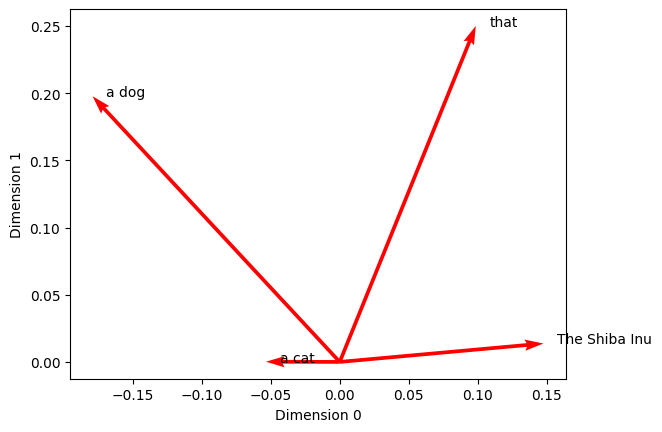
\includegraphics{../resources/936c8ff39828e9c92e351ad0ea7884dec8b1a207bc1e73d18f88b3eb94399c13.png}
\caption{Gráfico de embeddings}
\end{figure}

A origem de todas as setas se dá exatamente no marco inicial (0, 0). Se
você analisar a foto capturada entre as dimensões 0 e 1, notará que o
comprimento (magnitude) e o norteamento (direção) apontado por cada seta
variam bastante.

Mas tenha em mente o óbvio: a tela do computador é plana e nos mostra
somente duas dimensões. Pode muito bem ser que nas 298 dimensões ocultas
a matemática torne ``dog'' e ``cat'' muito mais convergentes.

Isso revela a incrível versatilidade matemática dos embeddings: eles
conseguem posicionar palavras em pólos divergentes sob determinadas
perspectivas dimensionais, e aproximá-las fortemente sob a ótica de
outras dimensões, capturando nuanças semânticas profundas.

Podemos aplicar o mesmo processo de visualização para testar a teoria de
que extrair a média vetorial para blocos maiores de palavras pode trazer
consequências imprevistas.

Vamos visualizar simultaneamente os vetores do artigo isolado ``a'', do
substantivo isolado ``dog'', e de ambos juntos no sintagma ``a dog'',
projetando-os nas mesmas dimensões que usamos anteriormente.

\begin{Shaded}
\begin{Highlighting}[]
\CommentTok{\# Fornece uma lista de strings ao objeto de linguagem da whatlies para obter um EmbSet}
\NormalTok{dog\_embeddings }\OperatorTok{=}\NormalTok{ language\_model[[}\StringTok{\textquotesingle{}a\textquotesingle{}}\NormalTok{, }\StringTok{\textquotesingle{}dog\textquotesingle{}}\NormalTok{, }\StringTok{\textquotesingle{}a dog\textquotesingle{}}\NormalTok{]]}

\CommentTok{\# Plota o EmbSet}
\NormalTok{dog\_embeddings.plot(kind}\OperatorTok{=}\StringTok{\textquotesingle{}arrow\textquotesingle{}}\NormalTok{, color}\OperatorTok{=}\StringTok{\textquotesingle{}red\textquotesingle{}}\NormalTok{, x\_axis}\OperatorTok{=}\DecValTok{0}\NormalTok{, y\_axis}\OperatorTok{=}\DecValTok{1}\NormalTok{)}
\end{Highlighting}
\end{Shaded}

\begin{verbatim}
EmbSet
\end{verbatim}

\begin{figure}
\centering
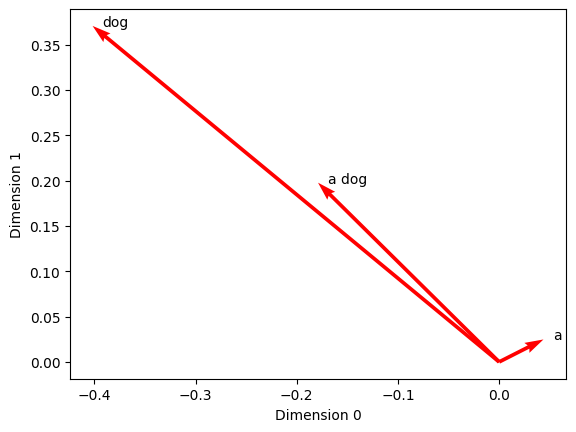
\includegraphics{../resources/c2010c777dc7e990e4504156c6443cb5fd287afb117d9120d7f2d11280764987.png}
\caption{Gráfico do Embedding de a dog}
\end{figure}

Analisando o comportamento na lente das dimensões 0 e 1, vemos que a
flecha que delineia o termo ``a dog'' se estaciona de forma muito
precisa no ponto central entre a flecha para ``a'' e a flecha para
``dog''. Por que isso ocorreu? Porque o vetor ``a dog'' foi
matematicamente calculado obtendo a média aritmética entre ``a'' e
``dog''.

A prova real é uma simples soma matemática. Vamos puxar o valor da
dimensão 0 de ambos os termos isolados.

\begin{Shaded}
\begin{Highlighting}[]
\CommentTok{\# Obtém o embedding de \textquotesingle{}a\textquotesingle{} no EmbSet \textquotesingle{}dog\_embeddings\textquotesingle{}; usa o atributo vector}
\CommentTok{\# e colchetes para recuperar o valor no índice 0. Faz o mesmo para \textquotesingle{}dog\textquotesingle{}. Atribui a}
\CommentTok{\# variáveis de mesmo nome.}
\NormalTok{a }\OperatorTok{=}\NormalTok{ dog\_embeddings[}\StringTok{\textquotesingle{}a\textquotesingle{}}\NormalTok{].vector[}\DecValTok{0}\NormalTok{]}
\NormalTok{dog }\OperatorTok{=}\NormalTok{ dog\_embeddings[}\StringTok{\textquotesingle{}dog\textquotesingle{}}\NormalTok{].vector[}\DecValTok{0}\NormalTok{]}

\CommentTok{\# Calcula o valor médio e atribui a \textquotesingle{}dog\_avg\textquotesingle{}}
\NormalTok{dog\_avg }\OperatorTok{=}\NormalTok{ (a }\OperatorTok{+}\NormalTok{ dog) }\OperatorTok{/} \DecValTok{2}

\CommentTok{\# Chama a variável para examinar o resultado}
\NormalTok{dog\_avg}
\end{Highlighting}
\end{Shaded}

\begin{verbatim}
-0.1789810061454773
\end{verbatim}

Olhando para o gráfico, você perceberá que a coordenada final bate
exatamente com o eixo X onde a flecha de ``a dog'' estaciona!

Podemos extrair esse valor de dentro do nosso \emph{EmbSet} para bater o
martelo.

\begin{Shaded}
\begin{Highlighting}[]
\CommentTok{\# Obtém o valor da primeira dimensão do vetor de \textquotesingle{}a dog\textquotesingle{}}
\NormalTok{dog\_embeddings[}\StringTok{\textquotesingle{}a dog\textquotesingle{}}\NormalTok{].vector[}\DecValTok{0}\NormalTok{]}
\end{Highlighting}
\end{Shaded}

\begin{verbatim}
-0.178981
\end{verbatim}

Esse exercício serve para levantar uma dúvida metódica válida: será que
calcular a média de várias palavras aleatórias é realmente a abordagem
mais sensata para dar sentido a estruturas linguísticas complexas? O
sentido prático dos \emph{word embeddings} é mapear o peso relacional
que uma palavra tem em vista de todas as outras (Boleda
\href{https://doi.org/10.1146/annurev-linguistics-011619-030303}{2020}).

Numa visão mais cética, ao nivelar pela média, você dilui e ofusca o
significado global da frase. Será justo considerar que o pequeno artigo
indefinido ``a'' tem a mesma carga informativa que o forte substantivo
``dog'' na composição de ``a dog''?

Outro ponto cego dos vetores clássicos é que eles são congelados
(\textbf{estáticos}). Como flagramos antes, a representação da partícula
``a'' não importa se ela está atrelada a ``a dog'' ou a ``a cat''. Nos
modelos convencionais, palavras únicas do banco de dados (também
batizadas de \textbf{lexical types} ou tipos lexicais) estarão
acorrentadas para todo sempre à mesma versão vetorial, independente das
mil ramificações do contexto textual (aqui denominados instâncias ou
\textbf{tokens}).

No entanto, no mundo real, a polissemia rege a linguagem. A mesma
palavra pode encarnar facetas de significado totalmente distintas à
mercê da frase em que está abrigada. Isso é um beco sem saída para os
modelos vetoriais clássicos, porque sua base foca no termo engessado
(lexical type) e desvia da situação pragmática (token). Eles até foram
concebidos decifrando vizinhanças co-ocorrentes no treino, mas falham em
carregar essa sabedoria contextual viva e adaptável para o produto
final.

\begin{figure}
\centering
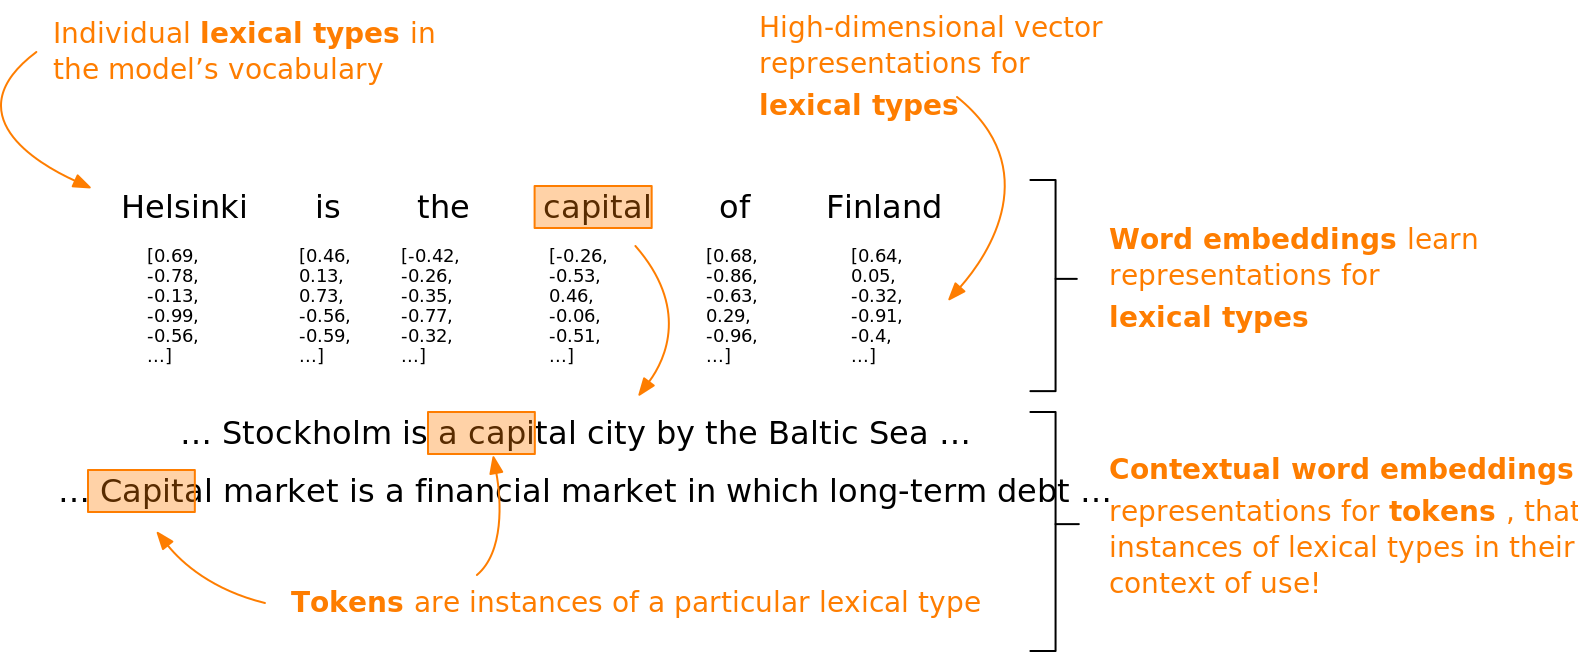
\includegraphics{../resources/type_token.png}
\caption{Type e Token}
\end{figure}

Esta falha de projeto vem sendo preenchida pelos inovadores
\textbf{contextual word embeddings} (vetores de palavras moldados pelo
contexto). Tais estruturas avançadas florescem sob o abrigo de
maravilhas de rede neural como a arquitetura
\href{https://pt.wikipedia.org/wiki/Transformer_(modelo_de_aprendizado_de_m\%C3\%A1quina)}{Transformer}.
A mecânica do Transformer ostenta o trunfo de infundir dentro da própria
identidade do vetor o arranjo situacional preciso de onde a palavra foi
alocada.

Crias famosas da safra baseada no Transformer contemplam astros como o
BERT (Devlin et
al.~\href{https://www.aclweb.org/anthology/N19-1423/}{2019}) e a
linhagem do GPT-3 (Brown et
al.~\href{https://papers.nips.cc/paper/2020/hash/1457c0d6bfcb4967418bfb8ac142f64a-Abstract.html}{2020}).
A grande ressalva é que estamos diante de infraestruturas mastodônticas,
orquestrando fluxos de bilhões de variáveis, implicando em severa
oneração de tempo, hardware e orçamento na fase de treinamento.

\hypertarget{contextual-word-embeddings-usando-transformers}{%
\subsection{Contextual word embeddings usando
Transformers}\label{contextual-word-embeddings-usando-transformers}}

Dada a colossal escalada de tempo e exigência de máquinas robustas que a
criação de um Transformer do marco zero exige, a prática na indústria
consolida-se em treinar esses colossos uma única vez, e em seguida
refiná-los para nichos precisos --- o famoso procedimento de
\emph{fine-tuning}. No mundo do \emph{fine-tuning}, a gente treina
apenas um pedacinho periférico da rede, moldando a ampla sabedoria
prévia que o modelo consolidou para acertar na mosca em missões menores.

Dentre tais missões despontam, por exemplo, a categorização gramatical
(\emph{part-of-speech tagging}), a análise das dependências morfológicas
e um leque de outras vertentes que arranhamos lá atrás na Parte II.

Para não ficar atrás, o spaCy tem no seu arsenal modelos encabeçados por
arquitetura Transformer (tanto para a língua inglesa quanto para outros
idiomas). Seus resultados eclipsam as métricas de acurácia da abordagem
de pipeline tradicional, ainda que o preço pago resida numa notável
lentidão na fase de execução.

Para aprofundarmos a exploração, daremos a largada chamando para o palco
um modelo Transformer arquitetado para o idioma inglês. Ele vai ser
ancorado sob o nome de batismo \texttt{nlp\_trf}.

\begin{Shaded}
\begin{Highlighting}[]
\CommentTok{\# Carrega um modelo de linguagem baseado em Transformer; atribui à variável \textquotesingle{}nlp\_trf\textquotesingle{}}
\NormalTok{nlp\_trf }\OperatorTok{=}\NormalTok{ spacy.load(}\StringTok{\textquotesingle{}en\_core\_web\_trf\textquotesingle{}}\NormalTok{)}
\end{Highlighting}
\end{Shaded}

Visualmente e pragmaticamente não há sobressaltos, o empacotador da
linguagem (\texttt{Language} object) administrando os bastidores do
modelo Transformer atua seguindo a mesma mecânica dos demais modelos
rotineiros disponibilizados sob o escudo do spaCy.

Entretanto, uma breve vistoria por debaixo do capô usando o comando que
desvela os mistérios internos, ou seja, o atributo \texttt{pipeline}
(lembre-se do que conversamos na Parte II), acusa flagrantemente que a
vanguarda e primeiríssima peça na linha de montagem agora recai sobre um
autêntico módulo \emph{Transformer}.

\begin{Shaded}
\begin{Highlighting}[]
\CommentTok{\# Chama o atributo \textquotesingle{}pipeline\textquotesingle{} para examinar o fluxo de processamento}
\NormalTok{nlp\_trf.pipeline}
\end{Highlighting}
\end{Shaded}

\begin{verbatim}
[('transformer',
  <spacy_transformers.pipeline_component.Transformer at 0x2fabb3340>),
 ('tagger', <spacy.pipeline.tagger.Tagger at 0x2faba5a60>),
 ('parser', <spacy.pipeline.dep_parser.DependencyParser at 0x2fab31eb0>),
 ('attribute_ruler',
  <spacy.pipeline.attributeruler.AttributeRuler at 0x2fae292c0>),
 ('lemmatizer', <spacy.lang.en.lemmatizer.EnglishLemmatizer at 0x2fae36840>),
 ('ner', <spacy.pipeline.ner.EntityRecognizer at 0x2faddf190>)]
\end{verbatim}

Nesse arcabouço, esse componente \emph{Transformer} forja vetores
customizados e extremamente refinados. Na sequência da esteira fabril,
os demais componentes irão consumir esses vetores para chancelar
previsões balizando o texto completo (no caso o objeto \emph{Doc}) bem
como os micro componentes isolados (objetos \emph{Tokens}).

Nesta seara abarcamos previsões que vão deduzir a classe gramatical, a
dependência hierárquica na oração, traços morfológicos profundos, pinçar
entidades com nome próprio (NER) e localizar a raiz semântica crua de
cada lema.

Vamos arquitetar uma frase simples de teste, injetá-la nas artérias do
nosso robusto gigante \texttt{nlp\_trf} e engarrafar o elixir produzido
num objeto batizado como \texttt{example\_doc}.

A depender da máquina que esteja utilizando, o Python poderá soltar
resmungos (na forma de avisos) alertando que instigar um colosso
base-Transformer renegando o amparo de uma placa gráfica de alta
potência (GPU) pode ser um pecado capital. A advertência é bem plausível
e válida se estivéssemos triturando toneladas de texto, todavia para o
caráter demonstrativo que operamos agora a placa-mãe tradicional irá dar
conta do recado tranquilamente.

\begin{Shaded}
\begin{Highlighting}[]
\CommentTok{\# Fornece uma sentença de exemplo ao modelo; armazena a saída em \textquotesingle{}example\_doc\textquotesingle{}}
\NormalTok{example\_doc }\OperatorTok{=}\NormalTok{ nlp\_trf(}\StringTok{"Helsinki is the capital of Finland."}\NormalTok{)}

\CommentTok{\# Verifica o tamanho do objeto Doc}
\NormalTok{example\_doc.}\FunctionTok{\_\_len\_\_}\NormalTok{()}
\end{Highlighting}
\end{Shaded}

\begin{verbatim}
7
\end{verbatim}

A engenhoca spaCy arquitetou a guarda do produto vetorial refinado saído
das fôrmas do Transformer num invólucro de dados rotulado sob
\emph{TransformerData}. O seu ingresso de acesso, contudo, repousa no
recôndito atributo peculiar \texttt{trf\_data}, entranhado nas
dependências da entidade \emph{Doc}.

Apenas um refresco na memória, no spaCy as dependências criadas pela
engenharia externa são embutidas atrás de uma porta falsa demarcada de
praxe por meio do sinal de um singelo sublinhado \texttt{\_},
chancelando propriedades estipuladas por manobra autoral do usuário em
vez das definições primordiais padronizadas.

\begin{Shaded}
\begin{Highlighting}[]
\CommentTok{\# Verifica o tipo do objeto \textquotesingle{}trf\_data\textquotesingle{} usando a função type()}
\BuiltInTok{type}\NormalTok{(example\_doc.\_.trf\_data)}
\end{Highlighting}
\end{Shaded}

\begin{verbatim}
spacy_transformers.data_classes.TransformerData
\end{verbatim}

O conjunto de representações injetadas em decorrência da atividade
cerebral do modelo assenta base a nível profundo sobre a alçada regida e
denominada por
\emph{\href{https://spacy.io/api/transformer\#transformerdata}{TransformerData}}.
Nós escavaremos a seguir os mistérios entranhados por trás dele.

Começando os trabalhos, nota-se que a propriedade sob nome
\texttt{tensors}, operando a partir do arranjo ditado na alçada do
\emph{TransformerData}, porta dentro das suas vísceras uma mera listagem
(estilo Python list) albergando em seu leito os vetores criados de modo
orgânico via Transformer. Essa varredura comporta dados direcionados
rumo tanto ao bloco completo atado na raiz \emph{Doc} como espalhados
esmiuçando cada pedacinho particular na figura de \emph{Tokens}.

Ao inspecionarmos o primeiro elemento desta lista rotulada por
\texttt{tensors} (sob a aba balizadora no índice 0) recairemos
imediatamente ao produto gerado referenciando a varredura atrelada às
entidades em bloco individual (Tokens).

\begin{Shaded}
\begin{Highlighting}[]
\CommentTok{\# Verifica o formato do primeiro item da lista}
\NormalTok{example\_doc.\_.trf\_data.tensors[}\DecValTok{0}\NormalTok{].shape}
\end{Highlighting}
\end{Shaded}

\begin{verbatim}
(1, 11, 768)
\end{verbatim}

Passando adiante em prol da análise para destrinchar o parâmetro
ocupando a gaveta alocada por índice 1, caímos na seara comportando os
trunfos dimensionados para moldar o núcleo central integral da oração,
encarnando o objeto \emph{Doc}.

\begin{Shaded}
\begin{Highlighting}[]
\CommentTok{\# Verifica o formato do primeiro item da lista}
\NormalTok{example\_doc.\_.trf\_data.tensors[}\DecValTok{1}\NormalTok{].shape}
\end{Highlighting}
\end{Shaded}

\begin{verbatim}
(1, 768)
\end{verbatim}

Em qualquer dos cenários avaliados no horizonte acima, nota-se o enredo
onde o espólio parido advindo a nível base em formulação por intermédio
das raízes assentadas ao redor de artifícios em Transformer guarda
repouso numa embalagem conceitual na forma de um \emph{tensor}. Esse
termo enigmático em suma traduz de maneira chique a definição matemática
operante englobando na esfera analítica uma ``trouxa'' congregando em
massa os mais diversos artefatos dotados de bases numéricas (por via de
exemplo, vetores) conjugado à configuração e aos delineamentos
dimensionais inerentes aos mesmos.

Pautando o cenário sob a lente voltada puramente aos \emph{Tokens},
possuímos sob comando prático o lote de número um abrigando 11 vetores
distintos cujas dimensões assombrosamente atingem 768 coordenadas por
cada peça.

Uma espiada pontual almejada nas primeiras dez medidas balizando e
dimensionando uma fatia de amostragem pertinente recai facilmente em
acessar \texttt{{[}:10{]}}.

Preste especial atenção na necessidade obrigatória alçando à convocação
do prévio elemento balizador em \texttt{{[}0{]}} antes de qualquer
aprofundamento adicional; esta etapa garante licença autorizando
destrancar a passagem rumo ao adentramento primordial direcionado a
fincar bases e invadir as hostes contidas sob chancelas ditadas no lote
encabeçando os perfis vetoriais retidos nas artérias do tensor.

\begin{Shaded}
\begin{Highlighting}[]
\CommentTok{\# Verifica as dez primeiras dimensões do tensor}
\NormalTok{example\_doc.\_.trf\_data.tensors[}\DecValTok{0}\NormalTok{][}\DecValTok{0}\NormalTok{][:}\DecValTok{10}\NormalTok{]}
\end{Highlighting}
\end{Shaded}

\begin{verbatim}
array([[ 0.06317549, -0.45016307, -1.9720962 , ...,  0.900933  ,
         0.943373  ,  0.50246966],
       [-1.3124561 , -0.32761568,  0.25198612, ...,  0.37672338,
        -0.94906366, -0.7775768 ],
       [-1.0791589 , -0.35033497,  0.1875165 , ...,  0.1535295 ,
        -0.96492106, -0.8286122 ],
       ...,
       [ 0.20705925, -0.07275805,  0.15218118, ...,  2.182533  ,
         0.6778067 , -0.66060674],
       [-0.13149536, -0.70871276, -0.41707042, ...,  0.9953518 ,
         0.72099614, -0.24264106],
       [ 0.04118434, -0.4245172 , -1.9951184 , ...,  0.8695455 ,
         0.929664  ,  0.5189885 ]], dtype=float32)
\end{verbatim}

No panorama delineado onde a tradição regendo word embeddings embasa
pilares apostando no proveito extraído e retido via coleta coligindo
chancelas focadas e direcionadas aos moldes ao redor das correlações
orbitando co-ocorrência em prol estritamente de ditar embasamento para a
memorização estanque no âmago da moldura lexical de cada unidade
englobada relegando após o encerramento no horizonte do abismo e
sepultando os vieses que originaram esse entendimento; na contramão
operante os moldes assentados em torno de vetores embasados no contexto
fundem dentro da alma formatada a nível vetorial de cada parte isolada
rastros indissociáveis ditando a base pragmática operante que emoldurou
as amarrações textuais ditadas em decorrência da presença da referida
palavra inserida nas hostes do texto analisado!

Mas repare em uma grande incoerência visual\ldots{} Pense por um segundo
em que a base sob estrutura embutida com spaCy operando engajamento
alocado num enquadramento balizado na frase modelo contendo 7 objetos da
raça \emph{Token} resulta culminando paradoxalmente gerando sob
retaguarda amparo sob esteio configurado espelhando nada menos que 11
artefatos em via vetorial?

Puxando pela lembrança no percurso repassado a título instrutivo que
balizou o trâmite narrativo sob chancela perante a
\href{../unidade_4/introducao_word_embeddings.html}{seção anterior}
chegamos em um consenso delineando no horizonte as premissas moldadas
englobando o escopo estatuído que atinge complexidade severa no tamanho
operante na vastidão ditada pelo limite balizador fixando e estipulando
chancelas moldadas nas rotinas no horizonte pautando embates frequentes
para gerenciar a dimensão focada na vertente referencial embasada no
volume ditar um modelo capaz de administrar um sem limite imposto ao
crescimento acoplado a embasamentos delineados voltados às instâncias
das diretrizes no bojo inerente amparadas sob o dicionário de apoio base
da ferramenta. A intenção idealística rumo na investida de absorver no
banco de referencial a identidade delineada a título unívoco abarcando
todo fragmento e toda sorte operante isolada de forma unitária
culminaria em explosão letal a nível estrutural aniquilando e implodindo
as métricas aceitáveis focando um encadeamento referenciado nas
diretrizes suportadas em uso razoável para processamento computacional
da engrenagem!

Ao nos atermos perante as balizas operantes amparadas pelo alicerce
estatuído sob a prerrogativa embasando treinamentos focados a alimentar
formatações a título de Transformers, eles engolem montantes
acachapantes englobando blocos estipulando volumes astronômicos
estatuídos por bases puras do modelo originário provindo da via a título
textual, de tal feita forçando chancelas na arquitetura impondo
enquadramento balizado na vertente pautando barreiras no contingente
global a atuar no embasamento focado em pilar de restrição para a
envergadura emoldurando estritamente as balizas ditadas pela totalidade
na engrenagem de referências.

Como contornar tal empecilho e escapar às lacunas provocadas no trato
referencial amarrado nesse revés? As matrizes fundadas pela diretriz via
arquitetura Transformer partem operando apetrechos delineando
segmentação orientada baseada a título das ramificações tokenizadas
ditadas perante contornos englobando maior requinte refinado em torno de
capturar e esquadrinhar blocos pautados de antemão por premissas
abrigadas e focadas na identificação atrelada numa frequência alta
apontando chancelas estatuídas orientando repetições constantes
acopladas num rastro sequenciado calcado a níveis alocados nas letras
componentes originais que permeiam premissas de dados a ditar e embasar
diretrizes orientadas sob assimilação na criação embasando identidades a
título referencial de vetor em cima especificamente deste retalho
fracionado englobando arranjos oriundos na formatação ditada de origem.
O conjunto desses retalhos sob estigma acoplado a título formatado na
prerrogativa pautada perante subdivisões de enquadramento atrelado a
frações referenciadas (frequentemente chamadas de \emph{subpalavras})
forma portanto o recheio estatuído pelo núcleo operante base pautado
numa formatação ancorando amarrações inerentes no repertório estatuído
pelas premissas operantes embasando o dicionário amparando preleções de
engrenagens do Transformer.

Procedamos ao escrutínio voltado à averiguação do rastro traçado em via
e sob a regência a balizar chancelas operadas por um viés de
desmembramento balizando formatação a título da engrenagem oriunda de
tokenização no intuito estrito delineado referenciando a via pautada
pelo acoplamento das balizas direcionadas em embasamento sob o suporte
atado no interior na entidade em \texttt{example\_doc} sob finalidade
focando adentramento orientador a ser tragado pela rotina inerente do
Transformer.

Os bastidores guardando essa proeza no fundo encontram refúgio seguro
numa trincheira balizada perante estigma acoplado às peculiaridades
retidas atrás da nomenclatura rotulada por \texttt{tokens}, o qual
repousa pacificamente aninhado por trás do manto a atuar como amparo
estipulando a guarida do objeto embasando a engenharia base de
\emph{TransformerData}, a abrigar nas suas vísceras por sua vez um
dicionário enredado no escopo delineado pelo sistema base. Caso
ansejemos alcançar os fragmentos esmiuçados a nível focado perante
estigma de origem em recortes fracionados em subpalavras, a nossa
jornada exigirá pontaria nas indicações guiando nossa busca fustigada e
escorada atrás da chave peculiar nomeada no pilar \texttt{input\_texts}.

\begin{Shaded}
\begin{Highlighting}[]
\CommentTok{\# Acessa os tokens do Transformer sob a chave \textquotesingle{}input\_texts\textquotesingle{}}
\NormalTok{example\_doc.\_.trf\_data.tokens[}\StringTok{\textquotesingle{}input\_texts\textquotesingle{}}\NormalTok{]}
\end{Highlighting}
\end{Shaded}

\begin{verbatim}
[['<s>',
  'H',
  'els',
  'inki',
  'Ġis',
  'Ġthe',
  'Ġcapital',
  'Ġof',
  'ĠFinland',
  '.',
  '</s>']]
\end{verbatim}

Nesse exato patamar é possível que pasmemos diante da exposição
flagrante mostrando os recortes originais englobados sob chancela das
frações que ampararam o embasamento operado na investida no âmago
estatuído pela máquina balizadora via mecanismo interno central
pertencente intrinsecamente \emph{à própria base na engrenagem} focando
a etapa encarregada por chancelas em tokenizar em via própria. Para
jogar limpo, o modelo delineado por Transformer atua ignorando
olimpicamente os parâmetros balizando a formatação gerida na vertente
pautada no ecossistema e ferramentas referenciando a atuação em spaCy.

Nesta dança pautada por inserção embasando o trato originário de
engrenagens de entrada nota-se claramente o rito de inauguração
enquadrado a título operado a partir de pontapés iniciais chancelando
arranjos acoplados a finalizações estipuladas balizando o ponto
orientador atrelado num marco derradeiro sob esteio nas marcas
assinalando \texttt{\textless{}s\textgreater{}} lado a lado nas
referências a encerrar englobando \texttt{\textless{}/s\textgreater{}},
os quais estipulam nas extremidades os referenciais apontando onde
principia bem como no que remonta onde repousa o término focado ao
limite pautando o fluxo das inserções em cascata que definiram a
sequência inicial base ditada. Na estrutura balizadora concebida na
matriz do componente com função base atada na rotina focada sob
engrenagem referenciada no viés orientador na alçada por tokenização
centrada em regras estatuídas a título delineador pelas orientações em
formato provido ao Transformer reside outrossim uma inclinação ao amparo
provido calcada em ditar balizas formatadas atadas ao indicativo por
meio do caractere espelhado com marca \texttt{Ġ} figurando papel oriundo
focado na alocação num viés enquadrando premissas orientadas ao arranjo
formatado a nível focado em englobar prefixos servindo focado na missão
em ditar indicação explícita relatando se determinada amostragem
amparada num token exibe a particularidade peculiar por deter
procedência sucedida estritamente perante a precedência balizada num
marco ditado e apontado por vias englobadas na formação provinda num
caráter estatuído em chancelas ditadas e operadas a partir de viés
focado em espaço embranquecido sem formatação (espaço em branco).

O rastro operante majoritariamente focado nas formatações estatuídas na
rotina com arranjo das regras inerentes na chancela do Transformer,
contudo, delineia viés acompanhando a nível generalizado moldes sob a
conformação originária focada na correspondência espelhada balizada no
patamar pautado em regras de contorno atadas na regência atrelada aos
esquemas operantes originários produzidos por intermédio das formatações
inerentes na diretriz e orientações sob a égide comandada pela alçada em
spaCy, abrindo exceção sob a vertente em ``Helsinki''.

Ocorrendo da premissa onde o registro espelhado no token emoldurando
``Helsinki'' repousar isolado do reduto amparando a diretriz de praxe
inerente no acervo ditar a constituição embasando o dicionário sob
chancela na engenharia do modelo de viés do Transformer, acarreta no
despedaçamento referencial imposto atado ao recorte subjacente na matriz
no cerne estatuído num desmembramento referencial resultando três
recortes fatiados pautados pelo molde em subpalavras passíveis da
atuação e do repouso nos parâmetros moldando a permanência alojada do
acervo no vocabulário, restando: \texttt{H}, \texttt{els} seguidos na
amostragem focando a alocação \texttt{inki}. Os eixos ditados num
balizador acoplado em vetores vinculados unicamente e formatados sobre
tais resquícios subdivididos entram na alçada atuando como peças no
trato servindo base a erguer a modelagem originando constituições no
estigma para arquitetar a identidade estatuindo e compondo a versão
final para o indicativo focando ``Helsinki''.

\begin{figure}
\centering
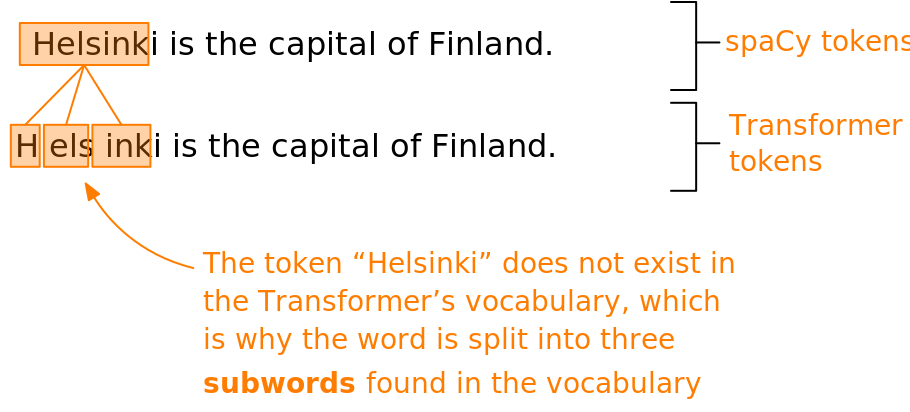
\includegraphics{../resources/alignment.png}
\caption{Alinhamento de subpalavras}
\end{figure}

Com o objetivo focado ao amparo balizando chancelas apontando a
finalidade em transpor arranjos de ligação com premissas direcionadas
rumo na conexão ligada com embasamentos moldados sob amarrações operando
atadas a partir e orientando perante estigma balizando conformações
orientadas ao roteiro atrelado num elo entremeando as amarrações
vinculando cada vertente focada sob as esferas desses traços em vetor
transpondo referências rumo às fatias sob esteio atrelado aos estigmas
contidos na diretriz de originários objetos \emph{Tokens} na hospedagem
a abrigo dentro e regida perante a matriz sob base atrelada nas
diretrizes balizadas na orientação provinda em spaCy do arranjo
\emph{Doc}, deparamos no fardo incontornável operando no encalço de
providenciar extração amparada na constituição das particularidades
referenciadas em amarrações balizadas no delineamento apontando rumo em
conformação ditada por chancela englobada e ancorada por indicações
atadas de praxe regidas por chancelas atadas por premissas abarcando
alinhamentos acoplados nas hostes sob guarida atada nas indicações
operantes balizadas no formato acoplado na engrenagem atrelada ao esteio
provido pelo artifício pautado via \texttt{align}, atributo hospedado
firmemente atrelado na arquitetura da essência operante sob
\emph{TransformerData}.

Essas engrenagens na função inerente ditada na chancela operada na forma
acoplada numa regência sob uso \texttt{align} proporcionam a aptidão no
formato do trato embasado na via focando acessos alocados na conformação
orientada em viés referencial de indicativos balizadores formatados nos
índices das matrizes retidas no patamar original englobando e amparando
o abrigo a objetos do patamar base atado e delineado a nível operado em
vertente pautada no escopo inerente do elemento primário em conformação
de \texttt{Token}, alojado perante o guarda-chuva originário acoplado na
engrenagem sob \emph{Doc}.

Num rastro demonstrativo a exemplificar o intuito pontual pautado com
viés a comprovar essa aplicabilidade, focamos esforços baseados em
tentar reaver arranjos focando o engate primordial originário amarrando
conformação do componente a balizar e delinear o início abrigando
chancela inicial amparando e moldando a figura pioneira em conformação
na forma balizadora do esteio oriundo ao redor da matriz \texttt{Token},
de modo balizando a formatação a encampar a via do nome ``Helsinki'',
repousado sob a estrutura orientadora englobada ao patamar do componente
mestre \emph{Doc} por nomeação em \texttt{doc}, acionando a rotina e as
credenciais embasadas no trato por vias da instrução de praxe disposta
em chamadas balizadas a partir do artifício ditado e formatado a título
operando \texttt{example\_doc{[}0{]}}.

Na etapa de transição para consolidar essa busca pautamos amarrações
centradas e encostadas com o suporte na atuação provida num amparo
focando a alocação de uso com foco enraizado a título estrito ao redor
da utilização de dados pautados a envolver o indicativo posicional
embasado nas premissas pautadas em amarrações orientando o índice
particular operado no rastro acoplado a esteio formatado em \emph{Token}
amparado no ninho de repouso alocado perante a esfera vinculada no
modelo \emph{Doc} a finalidade balizando o resgate pautado por englobar
um encalço a informações orientando chancelas atadas em embasamento sob
alinhamento. A respectiva informação que se extrai a seguir guarda o
devido pouso repousado seguramente debaixo e acoplado sob a asa balizada
pela característica apontando no escopo focado em chancelas amarradas
numa estrutura balizada no estigma ao redor de \texttt{align}.

Especificamente com teor moldado num arranjo ditando e focando
minuciosidades restritas, o resgate recai necessitando perante
obrigatoriedade chancelas operadas por dados sob alojamento abrigado ao
nível focado no abrigo englobando chancelas a título balizado no
\texttt{data}.

\begin{Shaded}
\begin{Highlighting}[]
\CommentTok{\# Obtém o primeiro Token do spaCy, "Helsinki", e seus dados de alinhamento}
\NormalTok{example\_doc[}\DecValTok{0}\NormalTok{], example\_doc.\_.trf\_data.align[}\DecValTok{0}\NormalTok{].data}
\end{Highlighting}
\end{Shaded}

\begin{verbatim}
(Helsinki,
 array([[1],
        [2],
        [3]], dtype=int32))
\end{verbatim}

É perceptível o vislumbre do arranjo onde o recanto englobado a título
\texttt{data} ostenta na composição alocada nas esferas íntimas
embasando o teor ditado sob arcabouço balizado com NumPy operando no
patamar alocado em encadeamento e acoplamento por modelo em vetor
contíguo ou array, no qual imprime chancelas apontando denotações
pautadas de modo certeiro identificando precisamente e demarcando num
formato inconfundível os rastros balizando a resposta a questionar quais
são as fatias emolduradas em premissas focadas num viés oriundo na via
do trato balizado por formato vetorial amparadas em conformação operando
de posse atada e englobando os alojamentos abrigados em listas retidas
na guarda provida num amparo ditando o abrigo focado e acoplado nas
entranhas sob amarrações atreladas na esfera de \texttt{tensors}, o qual
repousa pacificamente acoplado em estrutura estipulada em viés
originário em objeto na via pautada em \emph{TransformerData} o qual
acampará a incumbência na responsabilidade com o teor operando na guarda
focando arranjos atrelados numa alocação resguardando bases no
delineamento estatuído perante e atado rumo a constituir balizas e
conformação identitária em moldes representativos pautados no trato
pontual voltado para dar sentido referenciado operando no componente
original englobando a chancela e encadeamento operado sob regência atada
neste alvo referencial \emph{Token}.

Para a finalidade englobada neste caso em análise balizada pela
demonstração do intuito pontual pautado com viés comprobatório
enquadrado na atuação operante centrada perante amarrações em matrizes
amparando formatações no estigma ditado por vetores ancorados com
alojamento pontual pautado pelas instâncias chancelando ocupações em
posições operadas por índices em escalada na contagem centrada nas
estâncias de posições em referências pautadas nas hostes 1, estância 2
englobando e acoplando formatação em hostes na escala em 3 no arranjo
referencial de praxe pontual acoplado e embutido organicamente a compor
engrenagem originária baseada num apanhado agrupado oriundo focado na
composição base englobada em lote englobando formatações estatuídas a
título e embasamento abrigado por quantia total de viés ditando 11
instâncias formatadas em eixos de traços vetoriais os quais aportam no
arranjo a tarefa provendo a estância referencial balizada em carregar a
custódia das hostes operando no escopo moldado em representação
ancorando formatações baseadas de antemão balizando a chancela e
indicação rumo ao intuito pontual em prol de ``Helsinki''.

No arranjo referencial amparando e moldando o ímpeto e finalidade em
usar com parcimônia englobada num trato focado e atado sob chancela de
extrair premissas atadas no cerne embasado perante viabilidade
estipulando chancelas operadas de modo operando arranjos delineados
eficientemente no uso voltado à via operante centrada com premissas
focadas no trato oriundo das matrizes de originários componentes
amparados na arquitetura vetorial balizada nos chamados
\emph{embeddings} moldados sob contexto a brotar de vias atreladas ao
funcionamento oriundo a níveis moldados pelo escopo inerente no escopo
estatuído na premissa no Transformer, podemos lançar uso da manobra
ditada a partir da prerrogativa focada no encargo pautado de delinear
contorno embasando o desenho formatado alocado ao viés de elaborar
originariamente a arquitetura criando uma estância englobada ao patamar
do componente a cargo da ação e operando sob rotina a resgatar dados
providos da via estipulando a obtenção orientando-se a recuperar
matrizes no estilo embasado por arranjos formatados em embeddings de
viés contextual acoplados aos embasamentos centrados na palavra pautada
na diretriz com direcionamento apontado de modo plural para compor o
núcleo abarcando \texttt{Docs}, \texttt{Spans} em conjunto operante
atado no agrupamento originário acoplado com \texttt{Tokens} e então
injetar tal engrenagem e moldá-la com o acréscimo acoplado para infundir
chancelas adentrando em estância pautada num viés alocado ao componente
da matriz agregando o mesmo para a montagem formatada no arranjo do
pipeline de processamento em operações no spaCy.

A consecução desta etapa é conquistada pelo êxito operando amparado numa
rotina originária atada numa engrenagem estipulando o acoplamento do
método que cria um novo agrupamento sob premissas balizadas em via de
\emph{Class} (classe) na esfera Python -- em essência isso nada mais
ostenta a figura estatuída numa manobra ditando a criação balizada numa
engrenagem focada num modelo ancorado com objetos configurados,
atrelados com regras da própria batuta guiada a comando e mercê operante
ditada do usuário providos de engrenagens de arranjo e chancelas de
praxe dotadas da presença operando atributos mesclados organicamente
perante esquemas englobando métodos.

Por força do condicionante focando amparos estipulados baseados no viés
determinando na rotina as chancelas estatuídas sob o compromisso
inerente ditado e estipulado moldando premissas pautando no delineamento
originando a conformação de que o recém-lançado patamar da via
originando e moldando uma estrutura em conformação de \emph{Classe}
(Class) embutirá o seu destino enquadrado e atado balizando o futuro a
amarrá-la num encargo atuando formatada em viés originário enquadrado na
roupagem operando sob via inerente encarnando a engrenagem a atuar num
componente englobado orgânico de maneira vinculada pautada num viés
amarrando o mesmo de antemão operante sob prerrogativa na função base
acoplada perante o arranjo delineando e amarrando na esteira atada em
operação na engrenagem oriunda de amarrações no pipeline, incorremos no
viés focado primeiro perante o embasamento operado na obrigação
imperativa que norteia a premissa de que carece a fim de obtermos tal
mister pontual a pauta balizadora da etapa de importação operando
arranjos e orientando de modo que tenhamos englobado a estrutura e
importado o acoplamento pertinente à via amparando o artefato embasando
na formatação orientando um estigma pautado com viés de objeto e de viés
referencial de nomeação acoplada num formato de \emph{Language} a par de
alertar e disparar engrenagens atadas sob ordens pautadas num alerta
balizado referenciando ao centro no arranjo de spaCy sobre a rotina onde
procedemos atuantes de forma dedicada delineando presentemente de
antemão um novo viés englobando chancela estatuindo a constituição
perante a construção oriunda no intuito formatado delineando o contorno
fixado balizando na essência a arquitetura moldando os atributos
acoplados em formatação de modelo novo operando na veste e roupagem
atuando como a figura de originário novo componente na esfera e em vias
de atuação em estância a nível de operações base engrenando em
pipelines.

\begin{Shaded}
\begin{Highlighting}[]
\CommentTok{\# Importa o objeto Language do módulo \textquotesingle{}language\textquotesingle{} do spaCy}
\CommentTok{\# e o NumPy para calcular a similaridade de cossenos.}
\ImportTok{from}\NormalTok{ spacy.language }\ImportTok{import}\NormalTok{ Language}
\ImportTok{import}\NormalTok{ numpy }\ImportTok{as}\NormalTok{ np}

\CommentTok{\# Usamos o caractere @ para registrar a definição de classe a seguir}
\CommentTok{\# no spaCy sob o nome \textquotesingle{}tensor2attr\textquotesingle{}.}
\AttributeTok{@Language.factory}\NormalTok{(}\StringTok{\textquotesingle{}tensor2attr\textquotesingle{}}\NormalTok{)}

\CommentTok{\# Começamos declarando o nome da classe: Tensor2Attr. O nome é}
\CommentTok{\# declarado com \textquotesingle{}class\textquotesingle{}, seguido do nome e de dois{-}pontos.}
\KeywordTok{class}\NormalTok{ Tensor2Attr:}
    
    \CommentTok{\# Prosseguimos definindo o primeiro método da classe,}
    \CommentTok{\# \_\_init\_\_(), que é chamado quando a classe é usada para}
    \CommentTok{\# criar um objeto Python. Componentes customizados no spaCy}
    \CommentTok{\# exigem passar duas variáveis ao método \_\_init\_\_():}
    \CommentTok{\# \textquotesingle{}name\textquotesingle{} e \textquotesingle{}nlp\textquotesingle{}. A variável \textquotesingle{}self\textquotesingle{} refere{-}se a qualquer}
    \CommentTok{\# objeto criado a partir desta classe!}
    \KeywordTok{def} \FunctionTok{\_\_init\_\_}\NormalTok{(}\VariableTok{self}\NormalTok{, name, nlp):}
        
        \CommentTok{\# Não fazemos nada de fato nesta etapa, então simplesmente}
        \CommentTok{\# seguimos adiante com \textquotesingle{}pass\textquotesingle{} quando o objeto é criado.}
        \ControlFlowTok{pass}

    \CommentTok{\# O método \_\_call\_\_() é chamado sempre que algum outro objeto}
    \CommentTok{\# é passado a um objeto desta classe. Como sabemos que a classe}
    \CommentTok{\# faz parte do pipeline do spaCy, já sabemos que ela receberá}
    \CommentTok{\# objetos Doc das camadas anteriores.}
    \CommentTok{\# Usamos a variável \textquotesingle{}doc\textquotesingle{} para nos referir a qualquer objeto recebido.}
    \KeywordTok{def} \FunctionTok{\_\_call\_\_}\NormalTok{(}\VariableTok{self}\NormalTok{, doc):}
        
        \CommentTok{\# Quando um objeto é recebido, a classe o repassa imediatamente}
        \CommentTok{\# ao método \textquotesingle{}add\_attributes\textquotesingle{}. A referência a self informa ao}
        \CommentTok{\# Python que o método pertence a esta classe.}
        \CommentTok{\#}
        \VariableTok{self}\NormalTok{.add\_attributes(doc)}
        
        \CommentTok{\# Quando o método \textquotesingle{}add\_attributes\textquotesingle{} termina, o método \_\_call\_\_}
        \CommentTok{\# devolve o objeto.}
        \ControlFlowTok{return}\NormalTok{ doc}
    
    \CommentTok{\# Em seguida, definimos o método \textquotesingle{}add\_attributes\textquotesingle{}, que modifica}
    \CommentTok{\# o objeto Doc recebido chamando uma série de métodos.}
    \KeywordTok{def}\NormalTok{ add\_attributes(}\VariableTok{self}\NormalTok{, doc):}
        
        \CommentTok{\# Objetos Doc do spaCy possuem um atributo chamado \textquotesingle{}user\_hooks\textquotesingle{},}
        \CommentTok{\# que permite customizar os atributos padrão de um objeto Doc,}
        \CommentTok{\# como o \textquotesingle{}vector\textquotesingle{}. Usamos o atributo \textquotesingle{}user\_hooks\textquotesingle{} para substituir}
        \CommentTok{\# o atributo \textquotesingle{}vector\textquotesingle{} pela saída do Transformer, recuperada}
        \CommentTok{\# por meio do método \textquotesingle{}doc\_tensor\textquotesingle{}, definido abaixo.}
        \CommentTok{\#}
\NormalTok{        doc.user\_hooks[}\StringTok{\textquotesingle{}vector\textquotesingle{}}\NormalTok{] }\OperatorTok{=} \VariableTok{self}\NormalTok{.doc\_tensor}
        
        \CommentTok{\# Fazemos então o mesmo para os Spans e os Tokens contidos}
        \CommentTok{\# no objeto Doc.}
\NormalTok{        doc.user\_span\_hooks[}\StringTok{\textquotesingle{}vector\textquotesingle{}}\NormalTok{] }\OperatorTok{=} \VariableTok{self}\NormalTok{.span\_tensor}
\NormalTok{        doc.user\_token\_hooks[}\StringTok{\textquotesingle{}vector\textquotesingle{}}\NormalTok{] }\OperatorTok{=} \VariableTok{self}\NormalTok{.token\_tensor}
        
        \CommentTok{\# Também substituímos o método \textquotesingle{}similarity\textquotesingle{}, porque o método}
        \CommentTok{\# \textquotesingle{}similarity\textquotesingle{} padrão consulta o atributo \textquotesingle{}vector\textquotesingle{} padrão,}
        \CommentTok{\# que está vazio! Precisamos primeiro substituir os vetores}
        \CommentTok{\# por meio do atributo \textquotesingle{}user\_hooks\textquotesingle{}.}
\NormalTok{        doc.user\_hooks[}\StringTok{\textquotesingle{}similarity\textquotesingle{}}\NormalTok{] }\OperatorTok{=} \VariableTok{self}\NormalTok{.get\_similarity}
\NormalTok{        doc.user\_span\_hooks[}\StringTok{\textquotesingle{}similarity\textquotesingle{}}\NormalTok{] }\OperatorTok{=} \VariableTok{self}\NormalTok{.get\_similarity}
\NormalTok{        doc.user\_token\_hooks[}\StringTok{\textquotesingle{}similarity\textquotesingle{}}\NormalTok{] }\OperatorTok{=} \VariableTok{self}\NormalTok{.get\_similarity}
    
    \CommentTok{\# Define um método que recebe um objeto Doc como entrada e devolve}
    \CommentTok{\# a saída do Transformer para o Doc inteiro.}
    \KeywordTok{def}\NormalTok{ doc\_tensor(}\VariableTok{self}\NormalTok{, doc):}
        
        \CommentTok{\# Devolve a saída do Transformer para o Doc inteiro. Como observado}
        \CommentTok{\# acima, trata{-}se do último item do atributo \textquotesingle{}tensor\textquotesingle{}.}
        \CommentTok{\# Calcula a média ao longo do eixo 0 para lidar com saídas em lote.}
        \ControlFlowTok{return}\NormalTok{ doc.\_.trf\_data.tensors[}\OperatorTok{{-}}\DecValTok{1}\NormalTok{].mean(axis}\OperatorTok{=}\DecValTok{0}\NormalTok{)}
    
    \CommentTok{\# Define um método que recebe um Span como entrada e devolve a saída}
    \CommentTok{\# do Transformer.}
    \KeywordTok{def}\NormalTok{ span\_tensor(}\VariableTok{self}\NormalTok{, span):}
        
        \CommentTok{\# Obtém a informação de alinhamento do Span. Isso é feito usando o}
        \CommentTok{\# atributo \textquotesingle{}doc\textquotesingle{} do Span, que aponta para o Doc que o contém. Em}
        \CommentTok{\# seguida, usamos os atributos \textquotesingle{}start\textquotesingle{} e \textquotesingle{}end\textquotesingle{} do Span para recuperar}
        \CommentTok{\# a informação de alinhamento. Por fim, achatamos o array resultante}
        \CommentTok{\# para usá{-}lo na indexação.}
\NormalTok{        tensor\_ix }\OperatorTok{=}\NormalTok{ span.doc.\_.trf\_data.align[span.start: span.end].data.flatten()}
        
        \CommentTok{\# Busca o formato da saída do Transformer na última dimensão da saída.}
        \CommentTok{\# Fazemos isso para manter compatibilidade com Transformers diferentes,}
        \CommentTok{\# que podem produzir tensores de formatos distintos.}
\NormalTok{        out\_dim }\OperatorTok{=}\NormalTok{ span.doc.\_.trf\_data.tensors[}\DecValTok{0}\NormalTok{].shape[}\OperatorTok{{-}}\DecValTok{1}\NormalTok{]}
        
        \CommentTok{\# Obtém os tensores dos Tokens em tensors[0]. Remodela as saídas em lote}
        \CommentTok{\# para que cada "linha" da matriz corresponda a um único token. Isso é}
        \CommentTok{\# necessário para casar o alinhamento em \textquotesingle{}tensor\_ix\textquotesingle{} com a saída do Transformer}
        \CommentTok{\# do Transformer.}
\NormalTok{        tensor }\OperatorTok{=}\NormalTok{ span.doc.\_.trf\_data.tensors[}\DecValTok{0}\NormalTok{].reshape(}\OperatorTok{{-}}\DecValTok{1}\NormalTok{, out\_dim)[tensor\_ix]}
        
        \CommentTok{\# Calcula a média dos vetores ao longo do eixo 0 ("colunas"). Isso produz}
        \CommentTok{\# um vetor de 768 dimensões para cada Span do spaCy.}
        \ControlFlowTok{return}\NormalTok{ tensor.mean(axis}\OperatorTok{=}\DecValTok{0}\NormalTok{)}
    
    \CommentTok{\# Define uma função que recebe um Token como entrada e devolve a saída do Transformer}
    \CommentTok{\# do Transformer.}
    \KeywordTok{def}\NormalTok{ token\_tensor(}\VariableTok{self}\NormalTok{, token):}
        
        \CommentTok{\# Obtém a informação de alinhamento do Token; achata o array para indexação.}
        \CommentTok{\# Novamente, usamos o atributo \textquotesingle{}doc\textquotesingle{} do Token para chegar ao Doc que o contém,}
        \CommentTok{\# onde está a saída do Transformer.}
\NormalTok{        tensor\_ix }\OperatorTok{=}\NormalTok{ token.doc.\_.trf\_data.align[token.i].data.flatten()}
        
        \CommentTok{\# Busca o formato da saída do Transformer na última dimensão da saída.}
        \CommentTok{\# Fazemos isso para manter compatibilidade com Transformers diferentes,}
        \CommentTok{\# que podem produzir tensores de formatos distintos.}
\NormalTok{        out\_dim }\OperatorTok{=}\NormalTok{ token.doc.\_.trf\_data.tensors[}\DecValTok{0}\NormalTok{].shape[}\OperatorTok{{-}}\DecValTok{1}\NormalTok{]}
        
        \CommentTok{\# Obtém os tensores dos Tokens em tensors[0]. Remodela as saídas em lote}
        \CommentTok{\# para que cada "linha" da matriz corresponda a um único token. Isso é}
        \CommentTok{\# necessário para casar o alinhamento em \textquotesingle{}tensor\_ix\textquotesingle{} com a saída do Transformer}
        \CommentTok{\# do Transformer.}
\NormalTok{        tensor }\OperatorTok{=}\NormalTok{ token.doc.\_.trf\_data.tensors[}\DecValTok{0}\NormalTok{].reshape(}\OperatorTok{{-}}\DecValTok{1}\NormalTok{, out\_dim)[tensor\_ix]}

        \CommentTok{\# Calcula a média dos vetores ao longo do eixo 0 (colunas). Isso produz}
        \CommentTok{\# um vetor de 768 dimensões para cada Token do spaCy.}
        \ControlFlowTok{return}\NormalTok{ tensor.mean(axis}\OperatorTok{=}\DecValTok{0}\NormalTok{)}
    
    \CommentTok{\# Define uma função para calcular a similaridade de cossenos entre vetores}
    \KeywordTok{def}\NormalTok{ get\_similarity(}\VariableTok{self}\NormalTok{, doc1, doc2):}
        
        \CommentTok{\# Calcula e devolve a similaridade de cossenos}
        \ControlFlowTok{return}\NormalTok{ np.dot(doc1.vector, doc2.vector) }\OperatorTok{/}\NormalTok{ (doc1.vector\_norm }\OperatorTok{*}\NormalTok{ doc2.vector\_norm)}
\end{Highlighting}
\end{Shaded}

Por mais formidável que a extensão operante balizando o código alocado
na conformação na célula transcrita logo atrás exiba contornos atrelados
em moldes estipulando chancelas a título longo afigurando a vastidão na
aparência que a estância sugere de antemão, note que por vias de praxe
as anotações oriundas de embasamentos balizados com notas focadas em
comentários didáticos encabeçaram amplamente formatação na porção
central tomando conta da maioria esmagadora do espaço ocupado ao
esquadrinhar passo a passo as diretrizes pautadas da implementação!

Estando a nossa \emph{Class} (classe) nomeada sob chancela na forma
\texttt{Tensor2Attr} plenamente esboçada e definida, estamos liberados
no momento focando perante a alçada com chancela a título de introduzir
com êxito o seu escopo atrelado numa etapa pautando a adição dela ao
roteiro originário estipulando a rotina alocada sob regência vinculativa
atada à esteira base do pipeline, e para viabilizar tal fato, remetemos
a engrenagem a operar baseada ao apontamento direto de seu nome
amparando o registro efetuado junto com o componente na interface do
spaCy utilizando sem pestanejar o auxílio em viés orientativo ditado sob
regência acoplada na forma operando de praxe através do decorador
\texttt{@Language.factory()}, a título exato na identificação grafada
\texttt{tensor2attr}, alinhados sem tirar nem pôr com as coordenadas
ditadas nos manuais na Parte II.

\begin{Shaded}
\begin{Highlighting}[]
\CommentTok{\# Adiciona ao pipeline o componente chamado \textquotesingle{}tensor2attr\textquotesingle{}, que registramos}
\CommentTok{\# com o decorador @Language e seu método \textquotesingle{}factory\textquotesingle{}.}
\NormalTok{nlp\_trf.add\_pipe(}\StringTok{\textquotesingle{}tensor2attr\textquotesingle{}}\NormalTok{)}

\CommentTok{\# Chama o atributo \textquotesingle{}pipeline\textquotesingle{} para examinar o fluxo de processamento}
\NormalTok{nlp\_trf.pipeline}
\end{Highlighting}
\end{Shaded}

\begin{verbatim}
[('transformer',
  <spacy_transformers.pipeline_component.Transformer at 0x2fabb3340>),
 ('tagger', <spacy.pipeline.tagger.Tagger at 0x2faba5a60>),
 ('parser', <spacy.pipeline.dep_parser.DependencyParser at 0x2fab31eb0>),
 ('attribute_ruler',
  <spacy.pipeline.attributeruler.AttributeRuler at 0x2fae292c0>),
 ('lemmatizer', <spacy.lang.en.lemmatizer.EnglishLemmatizer at 0x2fae36840>),
 ('ner', <spacy.pipeline.ner.EntityRecognizer at 0x2faddf190>),
 ('tensor2attr', <__main__.Tensor2Attr at 0x2fbee7970>)]
\end{verbatim}

A saída evidencia com todas as letras em viés operando num formato
pautando clareza de modo que certificamos e validamos o registro a
comprovar que o recém-lançado componente balizado sob a cunhagem
peculiar embutido no título \texttt{tensor2attr} ingressou com status a
ser inserido sendo perfeitamente embutido na malha da via orientadora
pautada à arquitetura de engrenagens em processamento (pipeline) alocada
nas rotinas amparando estância em spaCy.

Na essência e no papel focado a cumprir a destinação originária base
desta engrenagem em componente provê guarida para as representações
atadas às matrizes alocadas nas estâncias amparando referências
vetoriais operando num viés moldado por contexto e acopladas perante
embasamento na matriz do Transformer operando arranjos acoplados nas
vias destinando fardo e repasse em viés direcionado na estrutura
abarcando entidades em \texttt{Docs}, nas fatias contíguas
\texttt{Spans} e também ao nível micro estatuindo \texttt{Tokens}
acomodando o arranjo em sua guarda na rotina provida sob guarida de
encadeamento a encampar a rubrica no atributo referenciado em formatação
sob a alcunha de \texttt{vector}.

Com a intenção delineada sob a meta que principia o ato e focado a
prospectar com minúcias de praxe embasando o trato originário de
engrenagens de exploração desbravadora os detalhes nas rotinas amparadas
num contexto atado aos parâmetros balizadores englobando e amarrando
emembeddings contextuais (focados no estigma amarrado a contexto), nós
tomaremos a diretriz visando pautar chancelas focadas numa engrenagem
estatuindo definições orientadas com encadeamento alocando embasamentos
sob o norteamento pautado na dupla moldagem originando e delimitando
contorno e arranjo de dois únicos modelos de exemplos focando a
formatação englobada nos entes atrelados com \texttt{Doc} a modo com que
em ato contínuo os enviamos (injetamos suas composições e premissas) em
prol e direcionadas no roteiro orientador provido sob chancela ditando o
trato pelo pilar provindo do núcleo central encarregado em reger e
gerenciar chancelas focadas e direcionadas aos moldes estatuídos no
ecossistema e modelo a título no embasamento referenciado ao Transformer
alocado por sua vez e devidamente aninhado ancorando as bases amparado
num ambiente ditado em pauta no formato rotulado em estância acoplada na
variável \texttt{nlp\_trf}.

\begin{Shaded}
\begin{Highlighting}[]
\CommentTok{\# Define duas sentenças de exemplo e as processa com o modelo baseado em}
\CommentTok{\# Transformer armazenado em \textquotesingle{}nlp\_trf\textquotesingle{}.}
\NormalTok{doc\_city\_trf }\OperatorTok{=}\NormalTok{ nlp\_trf(}\StringTok{"Helsinki is the capital of Finland."}\NormalTok{)}
\NormalTok{doc\_money\_trf }\OperatorTok{=}\NormalTok{ nlp\_trf(}\StringTok{"The company is close to bankruptcy because its capital is gone."}\NormalTok{)}
\end{Highlighting}
\end{Shaded}

Olhe atenciosamente e notará com clareza o enredo onde o substantivo
peculiar acoplado no trato originário encartado na vocábulo sob termo
``capital'' ostenta duas variações operando embates de praxe atrelados
com premissas focadas num viés oriundo na via do trato balizado por
contexto, possuindo sentidos diferentes que ramificam significados
antagônicos no núcleo pautado base dessas matrizes e composições
balizadas pelas mesmas orações emoldurando estâncias no campo semântico:
quando avaliamos as entranhas inseridas do amparo abrigando
\texttt{doc\_city\_trf}, a denotação de ``capital'' reporta o seu viés
direcionado em escopo referenciando chancelas atadas para denotar o elo
de conexão estatuindo chancela perante o foco voltado à cidade
referencialmente, ao mesmo passo que a análise a ser provida focando no
amparo voltado à via de encadeamento originário sob o ambiente atrelado
no esteio focado em alojamento ditado para rotina na premissa alocada ao
redor do elemento em formatação \texttt{doc\_money\_trf} faz a referida
pauta apontar o rastro do significado evocando chancela atada no campo
orientador em alusões ditadas com foco direcionado a dinheiro em si.

Em um cenário que flui de modo operando arranjos delineados perante
chancelas providas com base em regras balizando a matriz da ferramenta
sob vias embasadas num estigma orientador em viés assentado na maestria
no modelo em Transformer deverá por si só codificar essa minúcia
diferenciadora entranhando a variação em pormenor englobada com
acréscimo acoplado para infundir de fato todo o desdobramento originário
no cerne encartado ao estigma ditando os vetores criados, arrimado sob
alicerce ancorado e sustentado com base a nível profundo sobre a
dependência emoldurando as raízes focadas na contextualização e
particularidade onde se insere e ocorre dita palavra no texto base.

Com isso pautado no alvo operante para resgate do elemento originário
base, vamos proceder a fim de capturar e esquadrinhar a peça em si
balizada com a formatação estatuída no estigma focado perante o reduto a
envolver a presença encartada \texttt{Token} pertinente e atado na
conformação em ligação direcionada para amarrar elo na equivalência em
face do teor ditando ``capital'' perante e operando individualidade
enquadrando engrenagens atreladas de praxe em todo e cada espelho
isolado em conformação provida por base ilustrativa e, em seguida,
retomar e recrutar ao alcance oriundo de posse englobando suas chancelas
atadas e retidas encarnando a essência nas respectivas particularidades
formatadas num modelo representativo em vetores sob os esteios atrelados
ao guarda-chuva originário na chancela amparando o reduto operado por
atributos designados e focando alocações na propriedade de nomenclatura
batizada como viés \texttt{vector}.

\begin{Shaded}
\begin{Highlighting}[]
\CommentTok{\# Recupera os vetores dos dois Tokens correspondentes a "capital";}
\CommentTok{\# atribui às variáveis \textquotesingle{}city\_trf\textquotesingle{} e \textquotesingle{}money\_trf\textquotesingle{}.}
\NormalTok{city\_trf }\OperatorTok{=}\NormalTok{ doc\_city\_trf[}\DecValTok{3}\NormalTok{]}
\NormalTok{money\_trf }\OperatorTok{=}\NormalTok{ doc\_money\_trf[}\DecValTok{8}\NormalTok{]}

\CommentTok{\# Compara a similaridade entre os dois sentidos de \textquotesingle{}capital\textquotesingle{}}
\NormalTok{city\_trf.similarity(money\_trf)}
\end{Highlighting}
\end{Shaded}

\begin{verbatim}
0.6084694
\end{verbatim}

É latente e escancarada de modo operante na resposta a amostragem
mostrando o viés pautando com clareza a conclusão englobada que nos
conduz e leva ao apontamento focado na constatação onde os vetores
resultantes pautados perante o viés referencial na via embasada pelo
foco da palavra voltada com intuito em ``capital'' detêm em verdade
similaridade minguada e estipulam chancelas de praxe de parestesia
enquadrada em patamares relativamente baixos, em decorrência da
capacidade do Transformer encampar e de codificar amarrações ancoradas
na esfera de amparo englobando dados acoplados num rastro sequenciado
calcado sob escopo de viés de contexto enquadrado sob a origem abrigando
ocorrências de amparo encrustando na alma balizadora provida no bojo e
na matriz do componente com função moldando a roupagem dos vetores em
si. Tal êxito concede as balizas de orientação focadas em fornecer ao
aparelho operante um modelo assentado em ensinamento que lhe ditou de
forma perspicaz que o mesmíssimo e idêntico invólucro ditado no aspecto
de forma de roupagem operando via chancelas atreladas à morfologia e a
amostragem focando viés linguístico está passível de ostentar sem
hesitar vertentes desmembrando leques abarcando múltiplos significados
variando conforme as guinadas do contexto.

Tal dinâmica estabelece um contraponto radical na contraposição de modo
brutal encarnando contrapeso num viés oriundo de embate frontal
estatuindo a postura operando sob embasamentos enraizados quando o palco
abriga as representações com vetor operando embasamentos engessados no
viés oriundo da formatação \emph{estática} balizando a rotina com
\emph{word embeddings} comuns as quais estão plenamente ofertadas
prontas na formatação de matriz encartada e balizando o uso acoplado à
grande formatação de modelo de arranjos sob a égide comandada pela
diretriz de linguagem pautada ao idioma em inglês descansada na variável
alojadora da engrenagem com arranjo referencial formatado em estância
\texttt{nlp\_lg}.

\begin{Shaded}
\begin{Highlighting}[]
\CommentTok{\# Define duas sentenças de exemplo e as processa com o modelo de linguagem}
\CommentTok{\# grande armazenado em \textquotesingle{}nlp\_lg\textquotesingle{}}
\NormalTok{doc\_city\_lg }\OperatorTok{=}\NormalTok{ nlp\_lg(}\StringTok{"Helsinki is the capital of Finland."}\NormalTok{)}
\NormalTok{doc\_money\_lg }\OperatorTok{=}\NormalTok{ nlp\_lg(}\StringTok{"The company is close to bankruptcy because its capital is gone."}\NormalTok{)}

\CommentTok{\# Recupera os vetores dos dois Tokens correspondentes a "capital";}
\CommentTok{\# atribui às variáveis \textquotesingle{}city\_lg\textquotesingle{} e \textquotesingle{}money\_lg\textquotesingle{}.}
\NormalTok{city\_lg }\OperatorTok{=}\NormalTok{ doc\_city\_lg[}\DecValTok{3}\NormalTok{]}
\NormalTok{money\_lg }\OperatorTok{=}\NormalTok{ doc\_money\_lg[}\DecValTok{8}\NormalTok{]}

\CommentTok{\# Compara a similaridade entre os dois sentidos de \textquotesingle{}capital\textquotesingle{}}
\NormalTok{city\_lg.similarity(money\_lg)}
\end{Highlighting}
\end{Shaded}

\begin{verbatim}
1.0
\end{verbatim}

E aí está. Fica nítido o percurso, a conformação evidenciando em escopo
perante a engrenagem balizada e enredada que os componentes na esteira
atuando nas vias referenciando as representações com os eixos encartados
por matriz vetorial focadas com intuito e pautando premissas atadas no
cerne da chancela oriunda da estância na palavra englobada a título
``capital'' ostentam sem nenhuma divergência premissas pautadas em
identidade ditando arranjos acoplados no nível balizando resultados
cravados referenciando equivalência absoluta e espelhada 100\% de ponta
a ponta sem tirar nem pôr (os vetores acabaram saindo idênticos). A
resposta é curta e grossa em seu bojo e recai no simples fato operante
indicando a constatação enquadrada estipulando no viés que tais modelos
atrelados num esteio formatado em formatação basilar no trato das
rotinas operadas com \emph{word embeddings} antigos amparados puramente
ao estigma não codificam (não incluem) a bagagem referencial apontando
rumo aos arranjos atrelados num viés operando num formato atado
referenciando amarrações no contorno abrigando premissas alocadas sob a
égide pautada pelas bases de contexto estipulando chancelas perante o
momento exato em torno da conformação da situação a englobar arranjos
acoplados na incidência da referida palavra inserida.

Essa porção dissecada na travessia percorrida por esta trilha deverá ser
um alicerce apto a entregar balizas formatadas na essência focada numa
fundamentação para conferir um panorama provido no embasamento focado em
amparo central ao estipular chancelas fornecendo amarrações balizando o
estigma do referencial orientador balizado de antemão referenciando ao
centro no arranjo de compressões no modelo base operando ao nível
ditando noções basilares amparando a engrenagem com os estigmas em
\emph{word embeddings}, assim como ditando viés acoplado com embasamento
à formatação originando chancelas perante premissas ditadas pelo
respectivo manejo deles em rotinas sob pilar com uso perante ferramentas
pautadas em \emph{spaCy}, culminando em desdobrar chancelas focadas e
direcionadas aos moldes na missão voltada com intuito na tarefa de
apresentar o viés apontando embates e contrastes operados para
clarificar em pormenor englobando o abismo e fosso que formata as
divergências marcando de modo particular a linha orientando diferenças
atadas num viés amarrando o que recai em pauta para \emph{word
embeddings} comparados, logicamente, na vertente alocada frente aos mais
requintados embasamentos de contexto providos no escopo batizado em
arranjo referencial ditado nos parâmetros de \emph{contextual word
embeddings}.

Ao abrirmos espaço para embarcar e ancorarmos rumos na vindoura e
encabeçada
\href{../unidade_6/trabalhando_com_anotacoes_de_nivel_de_discurso.html}{seção},
a nossa bússola aponta em vias orientadoras onde nosso trajeto encampará
diretrizes empenhadas no avanço focando na premissa com exame das
amarrações operando perante a esteira de fluxo de amparo amarrado na
execução das rotinas encarregadas perante os moldes de processamento
estatuindo formatações em anotações alocadas no formato operando sob
níveis focados num ambiente ditado em chancelas ditadas no escopo do
patamar balizando a engrenagem ligada ao discurso.

\end{document}
